\chapter{定积分的应用}

\section{平面图形的面积}

在上一章开头讨论过由连续曲线 \(y = f\left( x\right) \left( { \geq  0}\right)\) ,以及直线 \(x = a,x = b\left( {a < b}\right)\) 和 \(x\) 轴所围曲边梯形的面积为
\[
A = {\int }_{a}^{b}f\left( x\right) \mathrm{d}x = {\int }_{a}^{b}y\mathrm{\;d}x.
\]
如果 \(f\left( x\right)\) 在 \(\left\lbrack  {a,b}\right\rbrack\) 上不都是非负的,则所围图形的面积为
\[
A = {\int }_{a}^{b}\left| {f\left( x\right) }\right| \mathrm{d}x = {\int }_{a}^{b}\left| y\right| \mathrm{d}x.
\]
一般地,由上、下两条连续曲线 \(y = {f}_{2}\left( x\right)\) 与 \(y = {f}_{1}\left( x\right)\) 以及两条直线 \(x = a\) 与 \(x = b(a <\) b) 所围的平面图形 (图 10-1), 它的面积计算公式为
\[
A = {\int }_{a}^{b}\left\lbrack  {{f}_{2}\left( x\right)  - {f}_{1}\left( x\right) }\right\rbrack  \mathrm{d}x. \tag{1}
\]
\begin{figure}
	\centering
	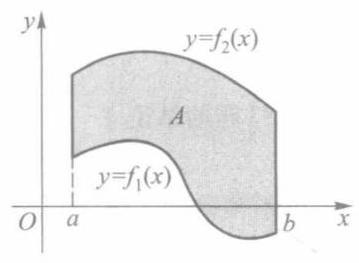
\includegraphics[width=.3\textwidth]{images/P065.jpg}
	\caption{图 $10-1$}
	\label{fig:P065}
\end{figure}

\begin{figure}
	\centering
	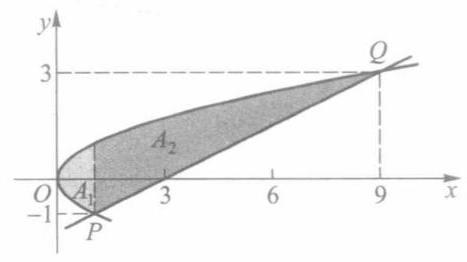
\includegraphics[width=.3\textwidth]{images/P066.jpg}
	\caption{图 $10-2$}
	\label{fig:P066}
\end{figure}

%例 1
\begin{example}

\end{example}
求由抛物线 \({y}^{2} = x\) 与直线 \(x - {2y} - 3 = 0\) 所围平面图形的面积 \(A\) .

%解
\begin{solution}

\end{solution}
该平面图形如图 10-2 所示. 先求出抛物线与直线的交点 \(P\left( {1, - 1}\right)\) 与 \(Q\left( {9,3}\right)\) . 用 \(x = 1\) 把图形分为左、右两部分,应用公式 (1) 分别求得它们的面积为
\[
{A}_{1} = {\int }_{0}^{1}\left\lbrack  {\sqrt{x} - \left( {-\sqrt{x}}\right) }\right\rbrack  \mathrm{d}x = 2{\int }_{0}^{1}\sqrt{x}\mathrm{\;d}x = \frac{4}{3},
\]
\[
{A}_{2} = {\int }_{1}^{9}\left( {\sqrt{x} - \frac{x - 3}{2}}\right) \mathrm{d}x = \frac{28}{3}.
\]
所以 \(A = {A}_{1} + {A}_{2} = \frac{32}{3}\) .

本题也可把抛物线方程和直线方程改写成
\[
x = {y}^{2} = {g}_{1}\left( y\right) ,x = {2y} + 3 = {g}_{2}\left( y\right) ,y \in  \left\lbrack  {-1,3}\right\rbrack  .
\]
并改取积分变量为 \(y\) ,便得
\[
A = {\int }_{-1}^{3}\left\lbrack  {{g}_{2}\left( y\right)  - {g}_{1}\left( y\right) }\right\rbrack  \mathrm{d}y
\]
\[
= {\int }_{-1}^{3}\left( {{2y} + 3 - {y}^{2}}\right) \mathrm{d}y = \frac{32}{3}\text{ . }
\]
设曲线 \(C\) 由参数方程
\[
x = x\left( t\right) ,y = y\left( t\right) ,t \in  \left\lbrack  {\alpha ,\beta }\right\rbrack   \tag{2}
\]
给出,在 \(\left\lbrack  {\alpha ,\beta }\right\rbrack\) 上 \(y\left( t\right)\) 连续, \(x\left( t\right)\) 连续可微且 \({x}^{\prime }\left( t\right)  \neq  0,t \in  \left( {\alpha ,\beta }\right)\) (对于 \(y\left( t\right)\) 连续可微且 \({y}^{\prime }\left( t\right)  \neq  0,t \in  \left( {\alpha ,\beta }\right)\) 的情形可类似地讨论). 记 \(a = x\left( \alpha \right) ,b = x\left( \beta \right) \left( {a < b\text{ 或 }b < a}\right)\) ,则由曲线 \(C\) 及直线 \(x = a,x = b\) 和 \(x\) 轴所围的图形,其面积计算公式为
\[
A = {\int }_{\alpha }^{\beta }\left| {y\left( t\right) {x}^{\prime }\left( t\right) }\right| \mathrm{d}t. \tag{3}
\]
%例 2
\begin{example}

\end{example}
求由摆线 \(x = a\left( {t - \sin t}\right) ,y = a\left( {1 - \cos t}\right) \left( {a > 0}\right)\) 的一拱与 \(x\) 轴所围平面图形 (图 10-3) 的面积.

\begin{figure}
	\centering
	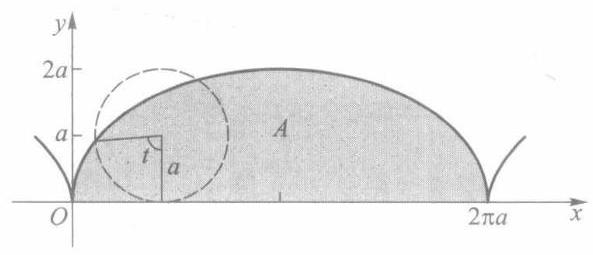
\includegraphics[width=.3\textwidth]{images/P067.jpg}
	\caption{图 $10-3$}
	\label{fig:P067}
\end{figure}

%解
\begin{solution}

\end{solution}
摆线的一拱可取 \(t \in  \left\lbrack  {0,{2\pi }}\right\rbrack\) . 所求面积为
\[
A = {\int }_{0}^{2\pi }a\left( {1 - \cos t}\right) {\left\lbrack  a\left( t - \sin t\right) \right\rbrack  }^{\prime }\mathrm{d}t
\]
\[
= {a}^{2}{\int }_{0}^{2\pi }{\left( 1 - \cos t\right) }^{2}\mathrm{\;d}t = {3\pi }{a}^{2}.
\]
如果由参数方程 (2) 所表示的曲线是封闭的, 即有
\[
x\left( \alpha \right)  = x\left( \beta \right) ,y\left( \alpha \right)  = y\left( \beta \right) ,
\]
且在 \(\left( {\alpha ,\beta }\right)\) 上曲线自身不再相交,那么由曲线自身所围图形的面积为
\[
A = \left| {{\int }_{\alpha }^{\beta }y\left( t\right) {x}^{\prime }\left( t\right) \mathrm{d}t}\right|
\]
\[
\left( \right. \text{ 或 }\left. \left| {{\int }_{\alpha }^{\beta }x\left( t\right) {y}^{\prime }\left( t\right) \mathrm{d}t}\right| \right) \text{ . } \tag{4}
\]
\begin{figure}
	\centering
	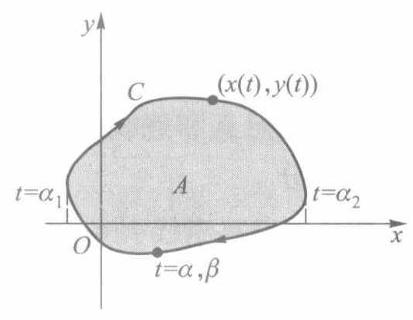
\includegraphics[width=.3\textwidth]{images/P068.jpg}
	\caption{图 $10-4$}
	\label{fig:P068}
\end{figure}

此公式可由公式 (1) 和 (3) 推出, 绝对值内的积分, 其正、负由曲线 (2) 的旋转方向所确定 (图 10-4).

%例 3
\begin{example}

\end{example}
求椭圆 \(\frac{{x}^{2}}{{a}^{2}} + \frac{{y}^{2}}{{b}^{2}} = 1\) 所围的面积.

%解
\begin{solution}

\end{solution}
化椭圆为参数方程
\[
x = a\cos t,y = b\sin t,t \in  \left\lbrack  {0,{2\pi }}\right\rbrack  .
\]
由公式 (4), 求得椭圆所围面积为
\[
A = \left| {{\int }_{0}^{2\pi }b\sin t{\left( a\cos t\right) }^{\prime }\mathrm{d}t}\right|
\]
\[
= {ab}{\int }_{0}^{2\pi }{\sin }^{2}t\mathrm{\;d}t = {\pi ab}.
\]
显然,当 \(a = b = r\) 时,这就等于圆面积 \(\pi {r}^{2}\) .

设曲线 \(C\) 由极坐标方程
\[
r = r\left( \theta \right) ,\theta  \in  \left\lbrack  {\alpha ,\beta }\right\rbrack
\]
给出,其中 \(r\left( \theta \right)\) 在 \(\left\lbrack  {\alpha ,\beta }\right\rbrack\) 上连续, \(\beta  - \alpha  \leq  {2\pi }\) . 由曲线 \(C\) 与两条射线 \(\theta  = \alpha ,\theta  = \beta\) 所围成的平面图形, 通常也称为扇形 (图 10-5). 此扇形的面积计算公式为
\[
A = \frac{1}{2}{\int }_{\alpha }^{\beta }{r}^{2}\left( \theta \right) \mathrm{d}\theta . \tag{5}
\]
\begin{figure}
	\centering
	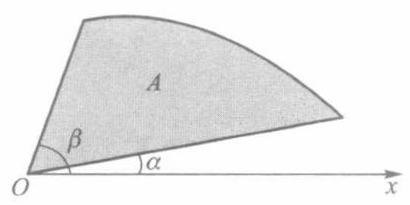
\includegraphics[width=.3\textwidth]{images/P069.jpg}
	\caption{图 $10-5$}
	\label{fig:P069}
\end{figure}

\begin{figure}
	\centering
	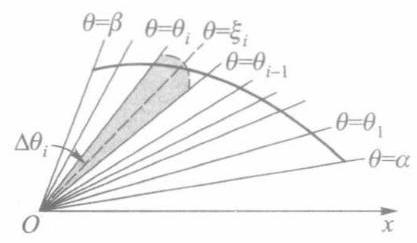
\includegraphics[width=.3\textwidth]{images/P070.jpg}
	\caption{图 $10-6$}
	\label{fig:P070}
\end{figure}

这仍可由定积分的基本思想而得. 如图 10-6 所示,对区间 \(\left\lbrack  {\alpha ,\beta }\right\rbrack\) 作任意分割
\[
T : \alpha  = {\theta }_{0} < {\theta }_{1} < \cdots  < {\theta }_{n - 1} < {\theta }_{n} = \beta ,
\]
射线 \(\theta  = {\theta }_{i}\left( {i = 1,2,\cdots ,n - 1}\right)\) 把扇形分成 \(n\) 个小扇形. 由于 \(r\left( \theta \right)\) 是连续的,因此当 \(\parallel T\parallel\) 很小时,在每一个 \({\Delta }_{i} = \left\lbrack  {{\theta }_{i - 1},{\theta }_{i}}\right\rbrack\) 上 \(r\left( \theta \right)\) 的值变化也很小. 任取 \({\xi }_{i} \in  {\Delta }_{i}\) ,便有
\[
r\left( \theta \right)  \approx  r\left( {\xi }_{i}\right) ,\theta  \in  {\Delta }_{i},i = 1,2,\cdots ,n.
\]
这时第 \(i\) 个小扇形的面积
\[
\Delta {A}_{i} \approx  \frac{1}{2}{r}^{2}\left( {\xi }_{i}\right) \Delta {\theta }_{i},
\]
于是
\[
A \approx  \mathop{\sum }\limits_{{i = 1}}^{n}\frac{1}{2}{r}^{2}\left( {\xi }_{i}\right) \Delta {\theta }_{i}.
\]
由定积分的定义和连续函数的可积性,当 \(\parallel T\parallel  \rightarrow  0\) 时,上式右边的极限即为公式 (5) 中的定积分.

%例 4
\begin{example}

\end{example}
求双纽线 \({r}^{2} = {a}^{2}\cos {2\theta }\) 所围平面图形的面积.

\begin{figure}
	\centering
	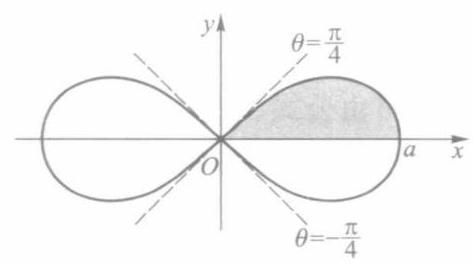
\includegraphics[width=.3\textwidth]{images/P071.jpg}
	\caption{图 $10-7$}
	\label{fig:P071}
\end{figure}

%解
\begin{solution}

\end{solution}
如图 10-7 所示,因为 \({r}^{2} \geq  0\) ,所以 \(\theta\) 的取值范围是 \(\left\lbrack  {-\frac{\pi }{4},\frac{\pi }{4}}\right\rbrack\) 与 \(\left\lbrack  {\frac{3\pi }{4},\frac{5\pi }{4}}\right\rbrack\) . 由图形的对称性及公式(5),得到
\[
A = 4 \cdot  \frac{1}{2}{\int }_{0}^{\frac{\pi }{4}}{a}^{2}\cos {2\theta }\mathrm{d}\theta  = {\left. {a}^{2}\sin 2\theta \right| }_{0}^{\frac{\pi }{4}} = {a}^{2}.
\]
\subsection{习题 10.1}

1. 求由抛物线 \(y = {x}^{2}\) 与 \(y = 2 - {x}^{2}\) 所围图形的面积.

2. 求由曲线 \(y = \left| {\ln x}\right|\) 与直线 \(x = \frac{1}{10},x = {10},y = 0\) 所围图形的面积.

3. 抛物线 \({y}^{2} = {2x}\) 把圆 \({x}^{2} + {y}^{2} \leq  8\) 分成两部分,求这两部分面积之比.

4. 求内摆线 \(x = a{\cos }^{3}t,y = a{\sin }^{3}t\left( {a > 0}\right)\) 所围图形的面积 (图 10-8).

\begin{figure}
	\centering
	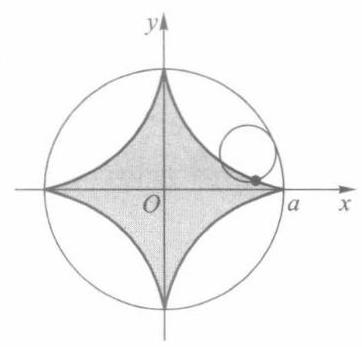
\includegraphics[width=.3\textwidth]{images/P072.jpg}
	\caption{图 $10-8$}
	\label{fig:P072}
\end{figure}

5. 求心形线 \(r = a\left( {1 + \cos \theta }\right) \left( {a > 0}\right)\) 所围图形的面积.

6. 求三叶形曲线 \(r = a\sin {3\theta }\left( {a > 0}\right)\) 所围图形的面积.

7. 求由曲线 \(\sqrt{\frac{x}{a}} + \sqrt{\frac{y}{b}} = 1\left( {a,b > 0}\right)\) 与坐标轴所围图形的面积. 8. 求由曲线 \(x = t - {t}^{3},y = 1 - {t}^{4}\) 所围图形的面积.

9. 求二曲线 \(r = \sin \theta\) 与 \(r = \sqrt{3}\cos \theta\) 所围公共部分的面积.

10. 求两椭圆 \(\frac{{x}^{2}}{{a}^{2}} + \frac{{y}^{2}}{{b}^{2}} = 1\) 与 \(\frac{{x}^{2}}{{b}^{2}} + \frac{{y}^{2}}{{a}^{2}} = 1\left( {a > 0,b > 0}\right)\) 所围公共部分的面积.

* 11. 证明: 对于由上、下两条连续曲线 \(y = {f}_{2}\left( x\right)\) 与 \(y = {f}_{1}\left( x\right)\) 以及两条直线 \(x = a\) 与 \(x = b\left( {a < b}\right)\) 所围的平面图形 \(A\) (图 10-1),存在包含 \(A\) 的多边形 \(\left\{  {U}_{n}\right\}\) 以及被 \(A\) 包含的多边形 \(\left\{  {W}_{n}\right\}\) ,使得当 \(n \rightarrow  \infty\) 时,它们的面积的极限存在且相等.

\section{由平行截面面积求体积}

设 \(\Omega\) 为三维空间中的一立体,它夹在垂直于 \(x\) 轴的两平面 \(x = a\) 与 \(x = b\) 之间 \(\left( {a < b}\right)\) . 为方便起见,称 \(\Omega\) 为位于 \(\left\lbrack  {a,b}\right\rbrack\) 上的立体. 若在任意一点 \(x \in  \left\lbrack  {a,b}\right\rbrack\) 处作垂直于 \(x\) 轴的平面,它截得 \(\Omega\) 的截面面积显然是 \(x\) 的函数,记为 \(A\left( x\right) ,x \in  \left\lbrack  {a,b}\right\rbrack\) ,并称之为 \(\Omega\) 的截面面积函数 (见图 10-9). 本节将导出由截面面积函数求立体体积的一般计算公式和旋转体的体积公式.

设截面面积函数 \(A\left( x\right)\) 是 \(\left\lbrack  {a,b}\right\rbrack\) 上的一个连续函数,且把 \(\Omega\) 的上述平行截面投影到某一垂直于 \(x\) 轴的平面上,它们永远是一个含在另一个的里面 \footnote{一般还可推广到 \(\Omega\) 由满足这种假设的若干个立体相加或相减而得的情形. 例如后面将要讨论的旋转体就是满足该条件的重要特例.}. 对 \(\left\lbrack  {a,b}\right\rbrack\) 作分割
\[
T : a = {x}_{0} < {x}_{1} < \cdots  < {x}_{n} = b.
\]


过各个分点作垂直于 \(x\) 轴的平面 \(x = {x}_{i},i = 1,2,\cdots ,n\) ,它们把 \(\Omega\) 切割成 \(n\) 个薄片 \({\Omega }_{i},i =\)  \(1,2,\cdots ,n\) . 任取 \({\xi }_{i} \in  \left\lbrack  {{x}_{i - 1},{x}_{i}}\right\rbrack\) ,那么每一薄片的体积 (见图 10-10).
\[
\Delta {V}_{i} \approx  A\left( {\xi }_{i}\right) \Delta {x}_{i}.
\]
于是
\[
V \approx  \mathop{\sum }\limits_{{i = 1}}^{n}A\left( {\xi }_{i}\right) \Delta {x}_{i}.
\]
\begin{figure}
	\centering
	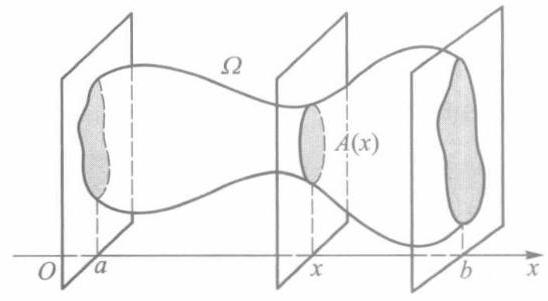
\includegraphics[width=.3\textwidth]{images/P073.jpg}
	\caption{图 $10-9$}
	\label{fig:P073}
\end{figure}

\begin{figure}
	\centering
	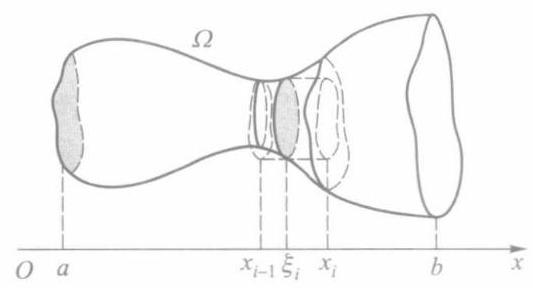
\includegraphics[width=.3\textwidth]{images/P074.jpg}
	\caption{图 $10-10$}
	\label{fig:P074}
\end{figure}

由定积分的定义和连续函数的可积性,当 \(\parallel T\parallel  \rightarrow  0\) 时,上式右边的极限存在,即为函数 \(A\left( x\right)\) 在 \(\left\lbrack  {a,b}\right\rbrack\) 上的定积分. 于是定义立体 \(\Omega\) 的体积为
\[
V = {\int }_{a}^{b}A\left( x\right) \mathrm{d}x. \tag{1}
\]
设 \(A\left( x\right)\) 在每个小区间 \({\Delta }_{i} = \left\lbrack  {{x}_{i - 1},{x}_{i}}\right\rbrack\) 上的最大、最小值分别为 \({M}_{i} = A\left( {\eta }_{i}\right)\) 与 \({m}_{i} =\)  \(A\left( {\zeta }_{i}\right)\) . 如果在这两个最大与最小截面上各作一高为 \(\Delta {x}_{i} = {x}_{i} - {x}_{i - 1}\) 的柱体 \({U}_{i}\) 和 \({W}_{i}\) ,则较大的一个 \({U}_{i}\) 将包含薄片 \({\Omega }_{i}\) ,而较小的一个 \({W}_{i}\) 将被薄片 \({\Omega }_{i}\) 所包含,那么每一薄片 \({\Omega }_{i}\) 的体积 \(\Delta {V}_{i}\) 满足
\[
{m}_{i}\Delta {x}_{i} \leq  \Delta {V}_{i} \leq  {M}_{i}\Delta {x}_{i}.
\]
于是, \(\Omega\) 的体积 \(V = \mathop{\sum }\limits_{{i = 1}}^{n}\Delta {V}_{i}\) 满足
\[
\mathop{\sum }\limits_{{i = 1}}^{n}{m}_{i}\Delta {x}_{i} \leq  V \leq  \mathop{\sum }\limits_{{i = 1}}^{n}{M}_{i}\Delta {x}_{i}.
\]
因为 \(A\left( x\right)\) 为连续函数,从而在 \(\left\lbrack  {a,b}\right\rbrack\) 上可积,所以极限
\[
\mathop{\lim }\limits_{{\parallel T\parallel  \rightarrow  0}}\mathop{\sum }\limits_{{i = 1}}^{n}{M}_{i}\Delta {x}_{i} = \mathop{\lim }\limits_{{\parallel T\parallel  \rightarrow  0}}\mathop{\sum }\limits_{{i = 1}}^{n}A\left( {\eta }_{i}\right) \Delta {x}_{i}\text{ 和 }\mathop{\lim }\limits_{{\parallel T\parallel  \rightarrow  0}}\mathop{\sum }\limits_{{i = 1}}^{n}{m}_{i}\Delta {x}_{i} = \mathop{\lim }\limits_{{\parallel T\parallel  \rightarrow  0}}\mathop{\sum }\limits_{{i = 1}}^{n}A\left( {\zeta }_{i}\right) \Delta {x}_{i}
\]
都存在,并且当 \(\parallel T\parallel\) 足够小时,能使
\[
\mathop{\sum }\limits_{{i = 1}}^{n}{\omega }_{i}\Delta {x}_{i} = \mathop{\sum }\limits_{{i = 1}}^{n}\left( {{M}_{i} - {m}_{i}}\right) \Delta {x}_{i} < \varepsilon ,
\]
其中 \(\varepsilon\) 为任意小的正数. 由此知道
\[
V = \mathop{\lim }\limits_{{\parallel T\parallel  \rightarrow  0}}\mathop{\sum }\limits_{{i = 1}}^{n}{M}_{i}\Delta {x}_{i} = \mathop{\lim }\limits_{{\parallel T\parallel  \rightarrow  0}}\mathop{\sum }\limits_{{i = 1}}^{n}{m}_{i}\Delta {x}_{i}.
\]
即: 对于立体 \(\Omega\) ,存在具有体积且包含 \(\Omega\) 的立体 \(U\left( T\right)  = \mathop{\bigcup }\limits_{{i = 1}}^{n}{U}_{i}\) 以及具有体积且被 \(\Omega\) 包含的立体 \(W\left( T\right)  = \mathop{\bigcup }\limits_{{i = 1}}^{n}{W}_{i}\) ,使得当 \(\parallel T\parallel  \rightarrow  0\) 时,它们的体积的极限存在且相等.

%例 1
\begin{example}

\end{example}
求由两个圆柱面 \({x}^{2} + {y}^{2} = {a}^{2}\) 与 \({z}^{2} + {x}^{2} = {a}^{2}\) 所围立体的体积.

\begin{figure}
	\centering
	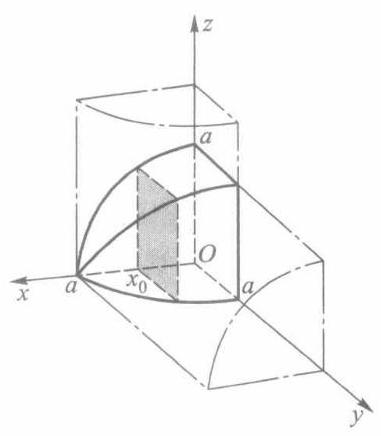
\includegraphics[width=.3\textwidth]{images/P075.jpg}
	\caption{图 $10-11$}
	\label{fig:P075}
\end{figure}

%解
\begin{solution}

\end{solution}
图 10-11 所示为该立体在第一卦限部分的图像 (占整体的八分之一). 对任一 \({x}_{0} \in  \left\lbrack  {0,a}\right\rbrack\) ,平面 \(x = {x}_{0}\) 与这部分立体的截面是一个边长为 \(\sqrt{{a}^{2} - {x}_{0}^{2}}\) 的正方形,所以 \(A\left( x\right)  = {a}^{2} - {x}^{2},x \in  \left\lbrack  {0,a}\right\rbrack\) . 由公式 (1) 便得
\[
V = 8{\int }_{0}^{a}\left( {{a}^{2} - {x}^{2}}\right) \mathrm{d}x = \frac{16}{3}{a}^{3}.
\]
%例 2
\begin{example}

\end{example}
求由椭球面 \(\frac{{x}^{2}}{{a}^{2}} + \frac{{y}^{2}}{{b}^{2}} + \frac{{z}^{2}}{{c}^{2}} = 1\) 所围立体 (椭球) 的体积.

%解
\begin{solution}

\end{solution}
以平面 \(x = {x}_{0}\left( {\left| {x}_{0}\right|  \leq  a}\right)\) 截椭球面,得椭圆 (它在 \({yOz}\) 平面上的正投影):
\[
\frac{{y}^{2}}{{b}^{2}\left( {1 - \frac{{x}_{0}^{2}}{{a}^{2}}}\right) } + \frac{{z}^{2}}{{c}^{2}\left( {1 - \frac{{x}_{0}^{2}}{{a}^{2}}}\right) } = 1.
\]
所以截面面积函数为 (根据 §1 例 3)
\[
A\left( x\right)  = {\pi bc}\left( {1 - \frac{{x}^{2}}{{a}^{2}}}\right) ,x \in  \left\lbrack  {-a,a}\right\rbrack  .
\]
于是求得椭球体积
\[
V = {\int }_{-a}^{a}{\pi bc}\left( {1 - \frac{{x}^{2}}{{a}^{2}}}\right) \mathrm{d}x = \frac{4}{3}{\pi abc}.
\]
显然,当 \(a = b = c = r\) 时,这就等于球的体积 \(\frac{4}{3}\pi {r}^{3}\) .

设 \({\Omega }_{A},{\Omega }_{B}\) 为位于同一区间 \(\left\lbrack  {a,b}\right\rbrack\) 上的两个立体,其体积分别为 \({V}_{A},{V}_{B}\) . 若在 \(\left\lbrack  {a,b}\right\rbrack\) 上它们的截面面积函数 \(A\left( x\right)\) 与 \(B\left( x\right)\) 皆连续,且 \(A\left( x\right)  = B\left( x\right)\) ,则由公式 (1) 推知 \({V}_{A} = {V}_{B}\) . 这个关于截面面积相等则体积也相等的原理, 早已为我国齐梁时代的数学家祖暅(祖冲之(429-500)之子,生卒年代约在公元 5 世纪末至 6 世纪初)在计算球的体积时所发现. 在《九章算术》一书中所记载的祖暅原理是:“夫叠基成立积, 缘幂势既同则积不容异”, 其中幂就是截面面积, 势就是高. 这就是说, 等高处的截面面积既然相等,则两立体的体积不可能不等 (图 10-12).17 世纪意大利数学家卡瓦列里 (Cavalieri) 也提出了类似的原理, 但要比祖暅晚一千一百多年.

\begin{figure}
	\centering
	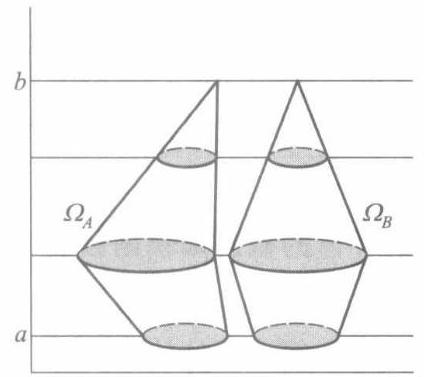
\includegraphics[width=.3\textwidth]{images/P076.jpg}
	\caption{图 $10-12$}
	\label{fig:P076}
\end{figure}

下面讨论旋转体的体积.

设 \(f\) 是 \(\left\lbrack  {a,b}\right\rbrack\) 上的连续函数, \(\Omega\) 是由平面图形
\[
0 \leq  \left| y\right|  \leq  \left| {f\left( x\right) }\right| ,a \leq  x \leq  b
\]
绕 \(x\) 轴旋转一周所得的旋转体. 那么易知截面面积函数为
\[
A\left( x\right)  = \pi {\left\lbrack  f\left( x\right) \right\rbrack  }^{2},x \in  \left\lbrack  {a,b}\right\rbrack  .
\]
由公式 (1),得到旋转体 \(\Omega\) 的体积公式为
\[
V = \pi {\int }_{a}^{b}{\left\lbrack  f\left( x\right) \right\rbrack  }^{2}\mathrm{\;d}x. \tag{2}
\]
%例 3
\begin{example}

\end{example}
试用公式 (2) 导出圆锥体的体积公式.

%解
\begin{solution}

\end{solution}
设正圆锥的高为 \(h\) ,底圆半径为 \(r\) . 如图 10-13 所示,这圆锥体可由平面图形 \(0 \leq  \left| y\right|  \leq  \frac{r}{h}x,x \in  \left\lbrack  {0,h}\right\rbrack\) 绕 \(x\) 轴旋转一周而得. 所以其体积为
\[
V = \pi {\int }_{0}^{h}{\left( \frac{r}{h}x\right) }^{2}\mathrm{\;d}x = \frac{1}{3}\pi {r}^{2}h,
\]
这个结果读者在中学课程里便已熟知了. 又因同底同高的两个圆锥, 在相同高度处的截面为相同的圆,即截面面积函数相同,所以任一高为 \(h\) ,底半径为 \(r\) 的圆锥 (正或斜), 其体积恒为 \(\frac{1}{3}\pi {r}^{2}h\) .

\begin{figure}
	\centering
	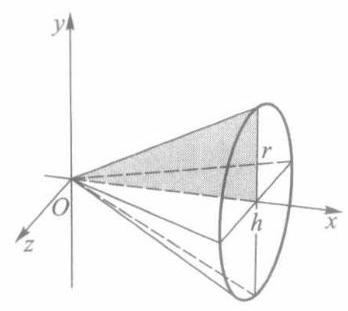
\includegraphics[width=.3\textwidth]{images/P077.jpg}
	\caption{图 $10-13$}
	\label{fig:P077}
\end{figure}

\begin{figure}
	\centering
	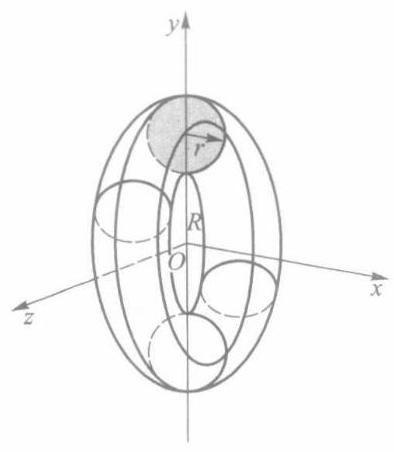
\includegraphics[width=.3\textwidth]{images/P078.jpg}
	\caption{图 $10-14$}
	\label{fig:P078}
\end{figure}

%例 4
\begin{example}

\end{example}
求由圆 \({x}^{2} + {\left( y - R\right) }^{2} \leq  {r}^{2}\left( {0 < r < R}\right)\) 绕 \(x\) 轴旋转一周所得环状立体的体积.

%解
\begin{solution}

\end{solution}
如图 10-14 所示,圆 \({x}^{2} + {\left( y - R\right) }^{2} = {r}^{2}\) 的上、下半圆分别为
\[
\begin{array}{l} y = {f}_{2}\left( x\right)  = R + \sqrt{{r}^{2} - {x}^{2}}, \\  y = {f}_{1}\left( x\right)  = R - \sqrt{{r}^{2} - {x}^{2}}, \end{array}\;\left| x\right|  \leq  r.
\]
故圆环体的截面面积函数是
\[
A\left( x\right)  = \pi {\left\lbrack  {f}_{2}\left( x\right) \right\rbrack  }^{2} - \pi {\left\lbrack  {f}_{1}\left( x\right) \right\rbrack  }^{2} = {4\pi R}\sqrt{{r}^{2} - {x}^{2}},x \in  \left\lbrack  {-r,r}\right\rbrack  .
\]
由此得到圆环体的体积为
\[
V = {8\pi R}{\int }_{0}^{r}\sqrt{{r}^{2} - {x}^{2}}\mathrm{\;d}x = 2{\pi }^{2}{r}^{2}R.
\]
如果把上述结果改写成 \(V = {2\pi R} \cdot  \pi {r}^{2}\) ,读者不难看出这相当于一个圆柱体的体积.

\subsection{习题 10.2}

1. 如图 10-15 所示, 直椭圆柱体被通过底面短轴的斜平面所截, 试求截得楔形体的体积.

2. 求下列平面曲线绕轴旋转所围成立体的体积:

\begin{figure}
	\centering
	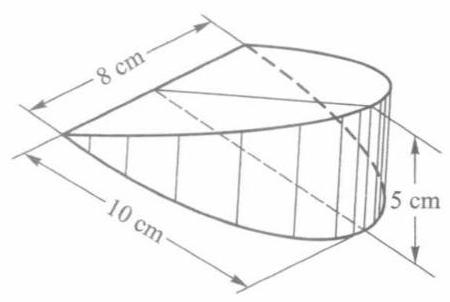
\includegraphics[width=.3\textwidth]{images/P079.jpg}
	\caption{图 $10-15$}
	\label{fig:P079}
\end{figure}

(1) \(y = \sin x,0 \leq  x \leq  \pi\) ,绕 \(x\) 轴；

(2) \(x = a\left( {t - \sin t}\right) ,y = a\left( {1 - \cos t}\right) \left( {a > 0}\right) ,0 \leq  t \leq  {2\pi }\) ,绕 \(x\) 轴；

(3) \(r = a\left( {1 + \cos \theta }\right) \left( {a > 0}\right)\) ,绕极轴；

(4) \(\frac{{x}^{2}}{{a}^{2}} + \frac{{y}^{2}}{{b}^{2}} = 1\) ,绕 \(y\) 轴.

3. 已知球半径为 \(r\) ,验证高为 \(h\) 的球缺体积 \(V =\)  \(\pi {h}^{2}\left( {r - \frac{h}{3}}\right) \left( {h \leq  r}\right) .\)

4. 求曲线 \(x = a{\cos }^{3}t,y = a{\sin }^{3}t\) 所围平面图形 (图 10-8) 绕 \(x\) 轴旋转所得立体的体积.

5. 导出曲边梯形 \(0 \leq  y \leq  f\left( x\right) ,a \leq  x \leq  b\) 绕 \(y\) 轴旋转所得立体的体积公式为
\[
V = {2\pi }{\int }_{a}^{b}{xf}\left( x\right) \mathrm{d}x.
\]
6. 求 \(0 \leq  y \leq  \sin x,0 \leq  x \leq  \pi\) 所示平面图形绕 \(y\) 轴旋转所得立体的体积.

\section{平面曲线的弧长与曲率}

\subsection{平面曲线的弧长}

先建立曲线弧长的概念.

设 \(C = \overset{⏜}{AB}\) 是一条没有自交点的非闭的平面曲线. 如图 10-16 所示,在 \(C\) 上从 \(A\) 到 \(B\) 依次取分点:
\[
A = {P}_{0},{P}_{1},{P}_{2},\cdots ,{P}_{n - 1},{P}_{n} = B,
\]
\begin{figure}
	\centering
	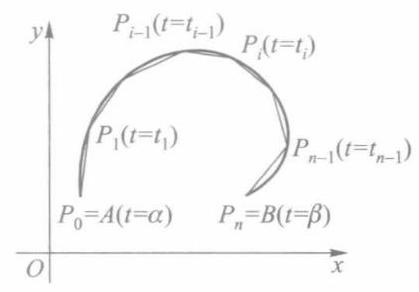
\includegraphics[width=.3\textwidth]{images/P080.jpg}
	\caption{图 $10-16$}
	\label{fig:P080}
\end{figure}

它们成为对曲线 \(C\) 的一个分割,记为 \(T\) . 然后用线段联结 \(T\) 中每相邻两点,得到 \(C\) 的 \(n\) 条弦 \(\overline{{P}_{i - 1}{P}_{i}}(i = 1\) , \(2,\cdots ,n)\) ,这 \(n\) 条弦又成为 \(C\) 的一条内接折线. 记
\[
\parallel T\parallel  = \mathop{\max }\limits_{{1 \leq  i \leq  n}}\left| {{P}_{i - 1}{P}_{i}}\right| ,\;{s}_{T} = \mathop{\sum }\limits_{{i = 1}}^{n}\left| {{P}_{i - 1}{P}_{i}}\right| ,
\]
分别表示最长弦的长度和折线的总长度.

%定义  1
\begin{definition}{}{def:}

\end{definition}
如果存在有限极限
\[
\mathop{\lim }\limits_{{\parallel T\parallel  \rightarrow  0}}{s}_{T} = s,
\]
即任给 \(\varepsilon  > 0\) ,恒存在 \(\delta  > 0\) ,使得对 \(C\) 的任何分割 \(T\) ,只要 \(\parallel T\parallel  < \delta\) ,就有
\[
\left| {{s}_{T} - s}\right|  < \varepsilon ,
\]
则称曲线 \(C\) 是可求长的,并把极限 \(s\) 定义为曲线 \(C\) 的弧长.

%定理 10.1
\begin{theorem}{}{the:}

\end{theorem}
 设曲线 \(C\) 是一条没有自交点的非闭的平面曲线,由参数方程
\[
x = x\left( t\right) ,\;y = y\left( t\right) ,\;t \in  \left\lbrack  {\alpha ,\beta }\right\rbrack   \tag{1}
\]
给出. 若 \(x\left( t\right)\) 与 \(y\left( t\right)\) 在 \(\left\lbrack  {\alpha ,\beta }\right\rbrack\) 上连续可微,则 \(C\) 是可求长的,且弧长为
\[
s = {\int }_{\alpha }^{\beta }\sqrt{{\left\lbrack  {x}^{\prime }\left( t\right) \right\rbrack  }^{2} + {\left\lbrack  {y}^{\prime }\left( t\right) \right\rbrack  }^{2}}\mathrm{\;d}t. \tag{2}
\]
%证
\begin{proof}

\end{proof}
如前所述,对 \(C\) 作任意分割 \(T = \left\{  {{P}_{0},{P}_{1},\cdots ,{P}_{n}}\right\}\) ,并设 \({P}_{0}\) 与 \({P}_{n}\) 分别对应 \(t = \alpha\) 与 \(t = \beta\) ,且
\[
{P}_{i}\left( {{x}_{i},{y}_{i}}\right)  = \left( {x\left( {t}_{i}\right) ,y\left( {t}_{i}\right) }\right) ,i = 1,2,\cdots ,n - 1.
\]
于是,与 \(T\) 对应地得到区间 \(\left\lbrack  {\alpha ,\beta }\right\rbrack\) 的一个分割
\[
{T}^{\prime } : \alpha  = {t}_{0} < {t}_{1} < {t}_{2} < \cdots  < {t}_{n - 1} < {t}_{n} = \beta .
\]
现在用反证法先证明 \(\mathop{\lim }\limits_{{\parallel T\parallel  \rightarrow  0}}\begin{Vmatrix}{T}^{\prime }\end{Vmatrix} = 0\) . 假设 \(\mathop{\lim }\limits_{{\parallel T\parallel  \rightarrow  0}}\begin{Vmatrix}{T}^{\prime }\end{Vmatrix} \neq  0\) ,则存在 \({\varepsilon }_{0} > 0\) ,对于任何 \(\delta  > 0\) ,都可以找到分割 \(T\) ,使得 \(\parallel T\parallel  < \delta\) ,而同时 \(\begin{Vmatrix}{T}^{\prime }\end{Vmatrix} \geq  {\varepsilon }_{0}\) ,从而可以找到 \(C\) 上两点 \({Q}^{\prime }\) 和 \({Q}^{\prime \prime }\) ,使得 \(\left| {{Q}^{\prime }{Q}^{\prime \prime }}\right|  < \delta\) ,而它们对应的参量 \({t}^{\prime }\) 和 \({t}^{\prime \prime }\) 满足 \(\left| {{t}^{\prime } - {t}^{\prime \prime }}\right|  \geq  {\varepsilon }_{0}\) . 依次取 \(\delta  = \frac{1}{n},n = 1\) , \(2,\cdots\) ,则得到两个点列 \(\left\{  {Q}_{n}^{\prime }\right\}\) 及 \(\left\{  {Q}_{n}^{\prime \prime }\right\}\) 和它们对应的参量数列 \(\left\{  {t}_{n}^{\prime }\right\}\) 及 \(\left\{  {t}_{n}^{\prime \prime }\right\}\) ,它们满足
\[
\left| {{Q}_{n}^{\prime }{Q}_{n}^{\prime \prime }}\right|  < \frac{1}{n},\;\left| {{t}_{n}^{\prime } - {t}_{n}^{\prime \prime }}\right|  \geq  {\varepsilon }_{0}.
\]
由致密性定理,存在子列 \(\left\{  {t}_{{n}_{k}}^{\prime }\right\}\) 及 \(\left\{  {t}_{{n}_{k}}^{\prime \prime }\right\}\) 和 \({t}^{ * },{t}^{* * } \in  \left\lbrack  {\alpha ,\beta }\right\rbrack\) ,使得
\[
\mathop{\lim }\limits_{{k \rightarrow  \infty }}{t}_{{n}_{k}}^{\prime } = {t}^{ * },\;\mathop{\lim }\limits_{{k \rightarrow  \infty }}{t}_{{n}_{k}}^{\prime \prime } = {t}^{* * }.
\]
显然, \(\left| {{t}^{ * } - {t}^{* * }}\right|  \geq  {\varepsilon }_{0}\) ,即 \({t}^{ * } \neq  {t}^{* * }\) . 设 \({t}^{ * }\) 和 \({t}^{* * }\) 对应的 \(C\) 上的点为 \({Q}^{ * }\) 和 \({Q}^{* * }\) ,则有 \(\left| {{Q}^{ * }{Q}^{* * }}\right|  = 0\) ,即两点重合. 这与 \(C\) 是一条没有自交点的非闭的曲线矛盾. 因此,当 \(\parallel T\parallel  \rightarrow  0\) 时 \(\begin{Vmatrix}{T}^{\prime }\end{Vmatrix} \rightarrow  0\) .

在 \({T}^{\prime }\) 所属的每个小区间 \({\Delta }_{i} = \left\lbrack  {{t}_{i - 1},{t}_{i}}\right\rbrack\) 上,由微分中值定理得
\[
\Delta {x}_{i} = x\left( {t}_{i}\right)  - x\left( {t}_{i - 1}\right)  = {x}^{\prime }\left( {\xi }_{i}\right) \Delta {t}_{i},{\xi }_{i} \in  {\Delta }_{i};
\]
\[
\Delta {y}_{i} = y\left( {t}_{i}\right)  - y\left( {t}_{i - 1}\right)  = {y}^{\prime }\left( {\eta }_{i}\right) \Delta {t}_{i},{\eta }_{i} \in  {\Delta }_{i}.
\]
从而曲线 \(C\) 的内接折线总长为
\[
{s}_{T} = \mathop{\sum }\limits_{{i = 1}}^{n}\sqrt{\Delta {x}_{i}^{2} + \Delta {y}_{i}^{2}} = \mathop{\sum }\limits_{{i = 1}}^{n}\sqrt{{\left\lbrack  {x}^{\prime }\left( {\xi }_{i}\right) \right\rbrack  }^{2} + {\left\lbrack  {y}^{\prime }\left( {\eta }_{i}\right) \right\rbrack  }^{2}}\Delta {t}_{i}.
\]
由于 \(\sqrt{{\left\lbrack  {x}^{\prime }\left( t\right) \right\rbrack  }^{2} + {\left\lbrack  {y}^{\prime }\left( t\right) \right\rbrack  }^{2}}\) 在 \(\left\lbrack  {\alpha ,\beta }\right\rbrack\) 上连续从而可积,因此根据定义 1,只需证明:
\[
\mathop{\lim }\limits_{{\parallel T\parallel  \rightarrow  0}}{s}_{T} = \mathop{\lim }\limits_{{\begin{Vmatrix}{T}^{\prime }\end{Vmatrix} \rightarrow  0}}\mathop{\sum }\limits_{{i = 1}}^{n}\sqrt{{\left\lbrack  {x}^{\prime }\left( {\xi }_{i}\right) \right\rbrack  }^{2} + {\left\lbrack  {y}^{\prime }\left( {\xi }_{i}\right) \right\rbrack  }^{2}}\Delta {t}_{i}, \tag{3}
\]
而后者即为 (2) 式右边的定积分. 为此记
\[
{\sigma }_{i} = \sqrt{{\left\lbrack  {x}^{\prime }\left( {\xi }_{i}\right) \right\rbrack  }^{2} + {\left\lbrack  {y}^{\prime }\left( {\eta }_{i}\right) \right\rbrack  }^{2}} - \sqrt{{\left\lbrack  {x}^{\prime }\left( {\xi }_{i}\right) \right\rbrack  }^{2} + {\left\lbrack  {y}^{\prime }\left( {\xi }_{i}\right) \right\rbrack  }^{2}},
\]
则有
\[
{s}_{T} = \mathop{\sum }\limits_{{i = 1}}^{n}\left\{  {\sqrt{{\left\lbrack  {x}^{\prime }\left( {\xi }_{i}\right) \right\rbrack  }^{2} + {\left\lbrack  {y}^{\prime }\left( {\xi }_{i}\right) \right\rbrack  }^{2}} + {\sigma }_{i}}\right\}  \Delta {t}_{i}.
\]
利用三角形不等式易证
\[
\left| {\sigma }_{i}\right|  \leq  \left| {{y}^{\prime }\left( {\eta }_{i}\right)  - {y}^{\prime }\left( {\xi }_{i}\right) }\right| ,i = 1,2,\cdots ,n.
\]
由 \({y}^{\prime }\left( t\right)\) 在 \(\left\lbrack  {\alpha ,\beta }\right\rbrack\) 上连续,从而一致连续,故对任给的 \(\varepsilon  > 0\) ,存在 \(\delta  > 0\) ,当 \(\begin{Vmatrix}{T}^{\prime }\end{Vmatrix} < \delta\) 时,只要 \({\xi }_{i},{\eta }_{i} \in  {\Delta }_{i}\) ,就有
\[
\left| {\sigma }_{i}\right|  < \frac{\varepsilon }{\beta  - \alpha },i = 1,2,\cdots ,n.
\]
因此有
\[
\left| {{s}_{T} - \mathop{\sum }\limits_{{i = 1}}^{n}\sqrt{{\left\lbrack  {x}^{\prime }\left( {\xi }_{i}\right) \right\rbrack  }^{2} + {\left\lbrack  {y}^{\prime }\left( {\xi }_{i}\right) \right\rbrack  }^{2}}\Delta {t}_{i}}\right|  = \left| {\mathop{\sum }\limits_{{i = 1}}^{n}{\sigma }_{i}\Delta {t}_{i}}\right|  \leq  \mathop{\sum }\limits_{{i = 1}}^{n}\left| {\sigma }_{i}\right| \Delta {t}_{i} < \varepsilon .
\]
即 (3) 式得证, 亦即公式 (2) 成立.

性质 设 \(\overset{⏜}{AB}\) 是一条没有自交点的非闭的可求长的平面曲线. 如果 \(D\) 是 \(\overset{⏜}{AB}\) 上一点, 则 \(\overset{⏜}{AD}\) 和 \(\overset{⏜}{DB}\) 也是可求长的,并且 \(\overset{⏜}{AB}\) 的弧长等于 \(\overset{⏜}{AD}\) 的弧长与 \(\overset{⏜}{DB}\) 的弧长的和.

该性质的证明这里从略 (参见本节习题 4 ).

%定义  2
\begin{definition}{}{def:}

\end{definition}
设曲线 \(\overset{⏜}{AB}\) 是一条没有自交点的闭的平面曲线. 在 \(\overset{⏜}{AB}\) 上任取一点 \(P\) 将 \(\overset{⏜}{AB}\) 分成两段非闭曲线,如果 \(\overset{⏜}{AP}\) 和 \(\overset{⏜}{PB}\) 都是可求长的,则称 \(\overset{⏜}{AB}\) 是可求长的,并把 \(\overset{⏜}{AP}\) 的弧长和 \(\overset{⏜}{PB}\) 的弧长的和定义为 \(\overset{⏜}{AB}\) 的弧长.

%注
\begin{remark}

\end{remark}
1 根据上述性质,显然定义 2 中 \(\overset{⏜}{AB}\) 是否可求长与 \(P\) 点的选取无关,并且当 \(\overset{⏜}{AB}\) 可求长时,其弧长也与 \(P\) 点的选取无关.

%注
\begin{remark}

\end{remark}
2 公式 (2) 也可以直接推广到有自交点的 (非) 闭的平面曲线的情形. 这里我们仅以 \(\overset{⏜}{AB}\) 是一条没有自交点的闭的平面曲线为例说明. 在 \(\overset{⏜}{AB}\) 上任取一点 \(P\) ,设 \(P\) 对应的参数为 \(\gamma  \in  \left( {\alpha ,\beta }\right)\) . 由定理 \({10.1},\overset{⏜}{AP}\) 和 \(\overset{⏜}{PB}\) 都是可求长的,且
\[
\overset{⏜}{AP}\text{ 的弧长 } = {\int }_{\alpha }^{\gamma }\sqrt{{\left\lbrack  {x}^{\prime }\left( t\right) \right\rbrack  }^{2} + {\left\lbrack  {y}^{\prime }\left( t\right) \right\rbrack  }^{2}}\mathrm{\;d}t,
\]
\[
\overset{⏜}{PB}\text{ 的弧长 } = {\int }_{\gamma }^{\beta }\sqrt{{\left\lbrack  {x}^{\prime }\left( t\right) \right\rbrack  }^{2} + {\left\lbrack  {y}^{\prime }\left( t\right) \right\rbrack  }^{2}}\mathrm{\;d}t\text{ , }
\]
从而 \(\overset{⏜}{AB}\) 是可求长的,且

\(\overset{⏜}{AB}\) 的弧长 \(= {\int }_{\alpha }^{\gamma }\sqrt{{\left\lbrack  {x}^{\prime }\left( t\right) \right\rbrack  }^{2} + {\left\lbrack  {y}^{\prime }\left( t\right) \right\rbrack  }^{2}}\mathrm{\;d}t + {\int }_{\gamma }^{\beta }\sqrt{{\left\lbrack  {x}^{\prime }\left( t\right) \right\rbrack  }^{2} + {\left\lbrack  {y}^{\prime }\left( t\right) \right\rbrack  }^{2}}\mathrm{\;d}t\)
\[
= {\int }_{\alpha }^{\beta }\sqrt{{\left\lbrack  {x}^{\prime }\left( t\right) \right\rbrack  }^{2} + {\left\lbrack  {y}^{\prime }\left( t\right) \right\rbrack  }^{2}}\mathrm{\;d}t.
\]
%定义  3
\begin{definition}{}{def:}

\end{definition}
设曲线 \(C\) 由参数方程 (1) 给出. 如果 \(x\left( t\right)\) 与 \(y\left( t\right)\) 在 \(\left\lbrack  {\alpha ,\beta }\right\rbrack\) 上连续可微,且 \({x}^{\prime }\left( t\right)\) 与 \({y}^{\prime }\left( t\right)\) 不同时为零 (即 \({x}^{\prime 2}\left( t\right)  + {y}^{\prime 2}\left( t\right)  \neq  0,t \in  \left\lbrack  {\alpha ,\beta }\right\rbrack\) ),则称 \(C\) 为一条光滑曲线.

推论 设曲线 \(C\) 由参数方程 (1) 给出. 若 \(C\) 为一条光滑曲线,则 \(C\) 是可求长的,且弧长为
\[
s = {\int }_{\alpha }^{\beta }\sqrt{{\left\lbrack  {x}^{\prime }\left( t\right) \right\rbrack  }^{2} + {\left\lbrack  {y}^{\prime }\left( t\right) \right\rbrack  }^{2}}\mathrm{\;d}t.
\]
若曲线 \(C\) 由直角坐标方程
\[
y = f\left( x\right) ,x \in  \left\lbrack  {a,b}\right\rbrack
\]
表示, 把它看作参数方程时, 即为
\[
x = x,y = f\left( x\right) ,x \in  \left\lbrack  {a,b}\right\rbrack  .
\]
所以当 \(f\left( x\right)\) 在 \(\left\lbrack  {a,b}\right\rbrack\) 上连续可微时,此曲线即为一光滑曲线. 这时弧长公式为
\[
s = {\int }_{a}^{b}\sqrt{1 + {f}^{\prime 2}\left( x\right) }\mathrm{d}x. \tag{4}
\]
又若曲线 \(C\) 由极坐标方程
\[
r = r\left( \theta \right) ,\theta  \in  \left\lbrack  {\alpha ,\beta }\right\rbrack
\]
表示, 把它化为参数方程, 则为
\[
x = r\left( \theta \right) \cos \theta ,y = r\left( \theta \right) \sin \theta ,\theta  \in  \left\lbrack  {\alpha ,\beta }\right\rbrack  .
\]
由于
\[
{x}^{\prime }\left( \theta \right)  = {r}^{\prime }\left( \theta \right) \cos \theta  - r\left( \theta \right) \sin \theta ,
\]
\[
{y}^{\prime }\left( \theta \right)  = {r}^{\prime }\left( \theta \right) \sin \theta  + r\left( \theta \right) \cos \theta ,
\]
\[
{x}^{\prime 2}\left( \theta \right)  + {y}^{\prime 2}\left( \theta \right)  = {r}^{2}\left( \theta \right)  + {r}^{\prime 2}\left( \theta \right) ,
\]
因此当 \({r}^{\prime }\left( \theta \right)\) 在 \(\left\lbrack  {\alpha ,\beta }\right\rbrack\) 上连续,且 \(r\left( \theta \right)\) 与 \({r}^{\prime }\left( \theta \right)\) 不同时为零时,此极坐标曲线为一光滑曲线. 这时弧长公式为
\[
s = {\int }_{\alpha }^{\beta }\sqrt{{r}^{2}\left( \theta \right)  + {r}^{\prime 2}\left( \theta \right) }\mathrm{d}\theta . \tag{5}
\]
%例 1
\begin{example}

\end{example}
求摆线 \(x = a\left( {t - \sin t}\right) ,y = a\left( {1 - \cos t}\right) \left( {a > 0}\right)\) 一拱的弧长 (见图 10-3).

%解
\begin{solution}

\end{solution}
\({x}^{\prime }\left( t\right)  = a\left( {1 - \cos t}\right) ,{y}^{\prime }\left( t\right)  = a\sin t\) ,由公式 (2) 得
\[
s = {\int }_{0}^{2\pi }\sqrt{{x}^{\prime 2}\left( t\right)  + {y}^{\prime 2}\left( t\right) }\mathrm{d}t = {\int }_{0}^{2\pi }\sqrt{2{a}^{2}\left( {1 - \cos t}\right) }\mathrm{d}t
\]
\[
= {2a}{\int }_{0}^{2\pi }\sin \frac{t}{2}\mathrm{\;d}t = {8a}.
\]
%例 2
\begin{example}

\end{example}
求悬链线 \(y = \frac{{\mathrm{e}}^{x} + {\mathrm{e}}^{-x}}{2}\) 从 \(x = 0\) 到 \(x = a > 0\) 那一段的弧长.

%解
\begin{solution}

\end{solution}
\({y}^{\prime } = \frac{{\mathrm{e}}^{x} - {\mathrm{e}}^{-x}}{2},1 + {y}^{\prime 2} = \frac{{\left( {\mathrm{e}}^{x} + {\mathrm{e}}^{-x}\right) }^{2}}{4}\) ,由公式 (4) 得
\[
s = {\int }_{0}^{a}\sqrt{1 + {y}^{\prime 2}}\mathrm{\;d}x = {\int }_{0}^{a}\frac{{\mathrm{e}}^{x} + {\mathrm{e}}^{-x}}{2}\mathrm{\;d}x = \frac{{\mathrm{e}}^{a} - {\mathrm{e}}^{-a}}{2}.
\]
%例 3
\begin{example}

\end{example}
求心形线 \(r = a\left( {1 + \cos \theta }\right) \left( {a > 0}\right)\) 的周长.

%解
\begin{solution}

\end{solution}
由公式 (5) 得
\[
s = {\int }_{0}^{2\pi }\sqrt{{r}^{2} + {r}^{\prime 2}}\mathrm{\;d}\theta  = 2{\int }_{0}^{\pi }\sqrt{2{a}^{2}\left( {1 + \cos \theta }\right) }\mathrm{d}\theta
\]
\[
= {4a}{\int }_{0}^{\pi }\cos \frac{\theta }{2}\mathrm{\;d}\theta  = {8a}.
\]
%注
\begin{remark}

\end{remark}
若把公式 (2) 中的积分上限改为 \(t\) ,就得到曲线 (1) 由端点 \({P}_{0}\) 到动点 \(P\left( {x\left( t\right) ,y\left( t\right) }\right)\) 的弧长,即
\[
s\left( t\right)  = {\int }_{\alpha }^{t}\sqrt{{x}^{\prime 2}\left( \tau \right)  + {y}^{\prime 2}\left( \tau \right) }\mathrm{d}\tau .
\]
由于被积函数是连续的, 因此
\[
\frac{\mathrm{d}s}{\mathrm{\;d}t} = \sqrt{{\left( \frac{\mathrm{d}x}{\mathrm{\;d}t}\right) }^{2} + {\left( \frac{\mathrm{d}y}{\mathrm{\;d}t}\right) }^{2}},
\]
\[
\mathrm{d}s = \sqrt{\mathrm{d}{x}^{2} + \mathrm{d}{y}^{2}}. \tag{6}
\]
特别称 \(s\left( t\right)\) 的微分 \(\mathrm{d}s\) 为弧微分. 如图 10-17 所示, \({PR}\) 为曲线在点 \(P\) 处的切线,在直角三角形 \({PQR}\) 中, \({PQ}\) 为 \(\mathrm{d}x,{QR}\) 为 \(\mathrm{d}y,{PR}\) 则为 \(\mathrm{d}s\) . 这个三角形称为微分三角形.

\subsection{曲率}

曲线上各点处的弯曲程度是描述曲线局部性态的又一重要标志.

考察图 10-18 中由参数方程 (1) 给出的光滑曲线 \(C\) . 我们看到弧段 \(\overset{⏜}{PQ}\) 与 \(\overset{⏜}{QR}\) 的长度相差不多而其弯曲程度却很不一样. 这反映为当动点沿曲线 \(C\) 从点 \(P\) 移至 \(Q\) 时,切线转过的角度 \({\Delta \alpha }\) 比动点从 \(Q\) 移至 \(R\) 时切线转过的角度 \({\Delta \beta }\) 要大得多.

设 \(\alpha \left( t\right)\) 表示曲线在点 \(P\left( {x\left( t\right) ,y\left( t\right) }\right)\) 处切线的倾角, \({\Delta \alpha } = \alpha \left( {t + {\Delta t}}\right)  - \alpha \left( t\right)\) 表示动点由 \(P\) 沿曲线移至 \(Q\left( {x\left( {t + {\Delta x}}\right) ,y\left( {t + {\Delta t}}\right) }\right)\) 时切线倾角的增量. 若 \(\overset{⏜}{PQ}\) 之长为 \({\Delta s}\) ,则称
\[
\bar{K} = \left| \frac{\Delta \alpha }{\Delta s}\right|
\]
\begin{figure}
	\centering
	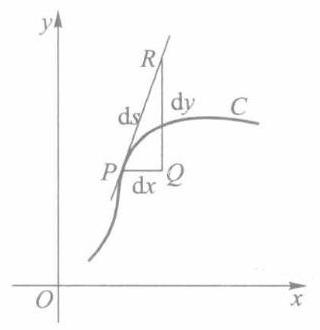
\includegraphics[width=.3\textwidth]{images/P081.jpg}
	\caption{图 $10-17$}
	\label{fig:P081}
\end{figure}

\begin{figure}
	\centering
	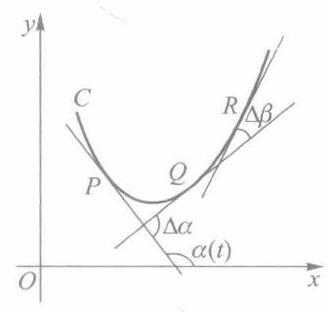
\includegraphics[width=.3\textwidth]{images/P082.jpg}
	\caption{图 $10-18$}
	\label{fig:P082}
\end{figure}

为弧段 \(\overset{⏜}{PQ}\) 的平均曲率. 如果存在有限极限
\[
K = \left| {\mathop{\lim }\limits_{{{\Delta t} \rightarrow  0}}\frac{\Delta \alpha }{\Delta s}}\right|  = \left| {\mathop{\lim }\limits_{{{\Delta s} \rightarrow  0}}\frac{\Delta \alpha }{\Delta s}}\right|  = \left| \frac{\mathrm{d}\alpha }{\mathrm{d}s}\right| ,
\]
则称此极限 \(K\) 为曲线 \(C\) 在点 \(P\) 处的曲率.

由于假设 \(C\) 为光滑曲线,故总有
\[
\alpha \left( t\right)  = \arctan \frac{{y}^{\prime }\left( t\right) }{{x}^{\prime }\left( t\right) }\text{ 或 }\alpha \left( t\right)  = \operatorname{arccot}\frac{{x}^{\prime }\left( t\right) }{{y}^{\prime }\left( t\right) }.
\]
又若 \(x\left( t\right)\) 与 \(y\left( t\right)\) 二阶可导,则由弧微分 (6) 可得
\[
\frac{\mathrm{d}\alpha }{\mathrm{d}s} = \frac{{\alpha }^{\prime }\left( t\right) }{{s}^{\prime }\left( t\right) } = \frac{{x}^{\prime }\left( t\right) {y}^{\prime \prime }\left( t\right)  - {x}^{\prime \prime }\left( t\right) {y}^{\prime }\left( t\right) }{{\left\lbrack  {x}^{\prime 2}\left( t\right)  + {y}^{\prime 2}\left( t\right) \right\rbrack  }^{3/2}}.
\]
所以曲率计算公式为
\[
K = \frac{\left| {x}^{\prime }{y}^{\prime \prime } - {x}^{\prime \prime }{y}^{\prime }\right| }{{\left( {x}^{\prime 2} + {y}^{\prime 2}\right) }^{3/2}}. \tag{7}
\]
若曲线由 \(y = f\left( x\right)\) 表示,则相应的曲率公式为
\[
K = \frac{\left| {y}^{\prime \prime }\right| }{{\left( 1 + {y}^{\prime 2}\right) }^{3/2}}. \tag{8}
\]
%例 4
\begin{example}

\end{example}
求椭圆 \(x = a\cos t,y = b\sin t,0 \leq  t \leq  {2\pi }\) 上曲率最大和最小的点.

%解
\begin{solution}

\end{solution}
由于 \({x}^{\prime } =  - a\sin t,{x}^{\prime \prime } =  - a\cos t,{y}^{\prime } = b\cos t,{y}^{\prime \prime } =  - b\sin t\) ,因此按公式 (7) 得椭圆上任意点处的曲率为
\[
K = \frac{ab}{{\left( {a}^{2}{\sin }^{2}t + {b}^{2}{\cos }^{2}t\right) }^{3/2}} = \frac{ab}{{\left\lbrack  \left( {a}^{2} - {b}^{2}\right) {\sin }^{2}t + {b}^{2}\right\rbrack  }^{3/2}}.
\]
当 \(a > b > 0\) 时,在 \(t = 0,\pi\) (长轴端点) 处曲率最大,而在 \(t = \frac{\pi }{2},\frac{3\pi }{2}\) (短轴端点) 处曲率最小, 且
\[
{K}_{\max } = \frac{a}{{b}^{2}},{K}_{\min } = \frac{b}{{a}^{2}}.
\]
若在例 4 中 \(a = b = R\) ,椭圆成为圆时,显然有
\[
K = \frac{1}{R},
\]
即在圆上各点处的曲率相同, 其值为半径的倒数.

容易知道, 直线上处处曲率为零.

设曲线 \(C\) 在其上一点 \(P\) 处的曲率 \(K \neq  0\) . 若过点 \(P\) 作一个半径为 \(\rho  = \frac{1}{K}\) 的圆,使它在点 \(P\) 处与曲线 \(C\) 有相同的切线,并在点 \(P\) 近旁与曲线位于切线的同侧 (图 10-19). 我们把这个圆称为曲线 \(C\) 在点 \(P\) 处的曲率圆或密切圆. 曲率圆的半径 \(\left( {\rho  = \frac{1}{K}}\right)\) 和圆心 \(\left( {P}_{0}\right)\) 称为曲线 \(C\) 在点 \(P\) 处的曲率半径和曲率中心. 由曲率圆的定义可以知道,曲线在点 \(P\) 与曲率圆既有相同的切线,又有相同的曲率和凸性.

\begin{figure}
	\centering
	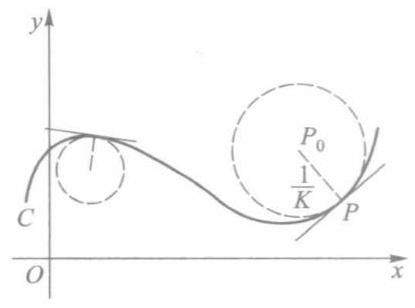
\includegraphics[width=.3\textwidth]{images/P083.jpg}
	\caption{图 $10-19$}
	\label{fig:P083}
\end{figure}

\begin{figure}
	\centering
	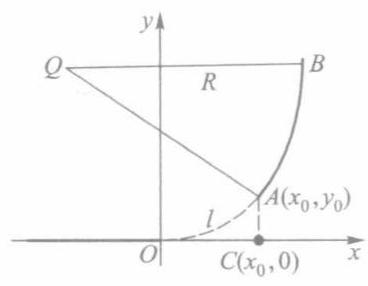
\includegraphics[width=.3\textwidth]{images/P084.jpg}
	\caption{图 $10-20$}
	\label{fig:P084}
\end{figure}

%例 5
\begin{example}

\end{example}
(铁路弯道分析) 如图 10-20 所示,火车轨道从直道进入到半径为 \(R\) 的圆弧形弯道时,为了行车安全,必须经过一段缓冲轨道(用虚线表示),使得曲率由零连续地增加到 \(\frac{1}{R}\) ,以保证火车的向心加速度 \(\left( {a = \frac{{v}^{2}}{\rho }}\right)\) 不发生跳跃性的突变.

图中 \(x\) 轴 \(\left( {x \leq  0}\right)\) 表示直线轨道, \(\overset{⏜}{AB}\) 是半径为 \(R\) 的圆弧形轨道 (点 \(Q\) 为其圆心), \(\overset{⏜}{OA}\) 为缓冲轨道. 我国一般采用的缓冲曲线是三次曲线
\[
y = \frac{{x}^{3}}{6Rl}, \tag{9}
\]
其中 \(l\) 是 \(\overset{⏜}{OA}\) 的弧长.

对曲线 (9) 应用曲率公式 (8) , 求得
\[
K = \frac{8{R}^{2}{l}^{2}x}{{\left( 4{R}^{2}{l}^{2} + {x}^{4}\right) }^{3/2}}.
\]
当 \(x\) 从 0 变为 \({x}_{0}\) 时,曲率 \(K\) 从 0 连续地变为
\[
{K}_{0} = \frac{8{R}^{2}{l}^{2}{x}_{0}}{{\left( 4{R}^{2}{l}^{2} + {x}_{0}^{4}\right) }^{3/2}} = \frac{1}{R} \cdot  \frac{8{l}^{2}{x}_{0}}{{\left( 4{l}^{2} + \frac{{x}_{0}^{4}}{{R}^{2}}\right) }^{3/2}}.
\]
当 \({x}_{0} \approx  l\) ,且 \(\frac{{x}_{0}}{R}\) 很小时, \({K}_{0} \approx  \frac{1}{R}\) . 因此曲线段 \(\overset{⏜}{OA}\) 的曲率从 0 逐渐增加到接近于 \(\frac{1}{R}\) ,从而起了缓冲作用.

\subsection{习题 10.3}



1. 求下列曲线的弧长:

\hspace*{1em} (1) \(y = {x}^{3/2},0 \leq  x \leq  4\) ;

\hspace*{1em} (2) \(\sqrt{x} + \sqrt{y} = 1\) ;

\hspace*{1em} (3) \(x = a{\cos }^{3}t,y = a{\sin }^{3}t\left( {a > 0}\right) ,0 \leq  t \leq  {2\pi }\) ;

\hspace*{1em} (4) \(x = a\left( {\cos t + t\sin t}\right) ,y = a\left( {\sin t - t\cos t}\right) \left( {a > 0}\right) ,0 \leq  t \leq  {2\pi }\) ;

\hspace*{1em} (5) \(r = a{\sin }^{3}\frac{\theta }{3}\left( {a > 0}\right) ,0 \leq  \theta  \leq  {3\pi }\) ；

\hspace*{1em} (6) \(r = {a\theta }\left( {a > 0}\right) ,0 \leq  \theta  \leq  {2\pi }\) .

* 2. 求下列各曲线在指定点处的曲率:

\hspace*{1em} (1) \({xy} = 4\) ,在点(2,2)；

\hspace*{1em} (2) \(y = \ln x\) ,在点(1,0)；

\hspace*{2em} (3) \(x = a\left( {t - \sin t}\right) ,y = a\left( {1 - \cos t}\right) \left( {a > 0}\right)\) ,在 \(t = \frac{\pi }{2}\) 的点;

\hspace*{1em} (4) \(x = a{\cos }^{3}t,y = a{\sin }^{3}t\left( {a > 0}\right)\) ,在 \(t = \frac{\pi }{4}\) 的点.



3. 求 \(a,b\) 的值,使椭圆 \(x = a\cos t,y = b\sin t\) 的周长等于正弦曲线 \(y = \sin x\) 在 \(0 \leq  x \leq  {2\pi }\) 上一段的长.

* 4. 本题的目的是证明性质 1. 这可按以下顺序逐一证明:

(1) 记 \(W = \left\{  {{s}_{T} \mid  T\text{ 是 }\overset{⏜}{AB}\text{ 的一个分割 }}\right\}\) ,则 \(W\) 是一个有界集.

(2)设 \(\overset{⏜}{AB}\) 的弧长为 \(s\) ,则 \(s = \sup W\) .

(3)记 \({W}^{\prime } = \left\{  {{s}_{{T}^{\prime }} \mid  {T}^{\prime }\text{ 是 }\overset{⏜}{AD}\text{ 的一个分割 }}\right\}\) 及 \({W}^{\prime \prime } = \left\{  {{s}_{{T}^{\prime \prime }} \mid  {T}^{\prime \prime }\text{ 是 }\overset{⏜}{DB}\text{ 的一个分割 }}\right\}\) ,则 \({W}^{\prime }\) 和 \({W}^{\prime \prime }\) 都是有界集,并且如果记 \({s}^{\prime } = \sup {W}^{\prime }\) 及 \({s}^{\prime \prime } = \sup {W}^{\prime \prime }\) ,则
\[
s = {s}^{\prime } + {s}^{\prime \prime }.
\]
(4) 证明: \(\overset{⏜}{AD}\) 的弧长为 \({s}^{\prime },\overset{⏜}{DB}\) 的弧长为 \({s}^{\prime \prime }\) .

5. 设曲线由极坐标方程 \(r = r\left( \theta \right)\) 给出,且二阶可导,证明它在点 \(\left( {r,\theta }\right)\) 处的曲率为
\[
K = \frac{\left| {r}^{2} + 2{r}^{\prime 2} - r{r}^{\prime \prime }\right| }{{\left( {r}^{2} + {r}^{\prime 2}\right) }^{3/2}}.
\]
6. 用上题公式,求心形线 \(r = a\left( {1 + \cos \theta }\right) \left( {a > 0}\right)\) 在 \(\theta  = 0\) 处的曲率、曲率半径和曲率圆.

7. 证明抛物线 \(y = a{x}^{2} + {bx} + c\) 在顶点处的曲率为最大.

* 8. 求曲线 \(y = {\mathrm{e}}^{x}\) 上曲率最大的点.

\section{旋转曲面的面积}

定积分的所有应用问题,一般总可按“分割,近似求和,取极限”三个步骤导出所求量的积分形式. 但为简便实用起见, 也常采用下面介绍的 “微元法”. 本节和下一节将采用此法来处理.

\subsection{微元法}

在上一章我们已经熟知,若令 \(\Phi \left( x\right)  = {\int }_{a}^{x}f\left( t\right) \mathrm{d}t\) ,则当 \(f\) 为连续函数时, \({\Phi }^{\prime }\left( x\right)  =\)  \(f\left( x\right)\) ,或 \(\mathrm{d}\Phi  = f\left( x\right) \mathrm{d}x\) ,且
\[
\Phi \left( a\right)  = 0,\;\Phi \left( b\right)  = {\int }_{a}^{b}f\left( x\right) \mathrm{d}x.
\]
现在恰好要把问题倒过来: 如果所求量 \(\Phi\) 是分布在某区间 \(\left\lbrack  {a,x}\right\rbrack\) 上的,或者说它是该区间端点 \(x\) 的函数,即 \(\Phi  = \Phi \left( x\right) ,x \in  \left\lbrack  {a,b}\right\rbrack\) ,而且当 \(x = b\) 时, \(\Phi \left( b\right)\) 适为最终所求的值.

在任意小区间 \(\left\lbrack  {x,x + {\Delta x}}\right\rbrack   \subset  \left\lbrack  {a,b}\right\rbrack\) 上,恰当选取 \(\Phi\) 的微小增量 \({\Delta \Phi }\) 的近似可求量 \({\Delta }^{\prime }\Phi\) (所谓 \({\Delta \Phi }\) 的近似可求量是指用来近似代替 \({\Delta \Phi }\) 的有确定意义而且可以计算的量. 例如: 当 \(\Phi\) 是由函数 \(f\) 确定的曲边梯形的面积时, \({\Delta }^{\prime }\Phi\) 是以 \(f\left( x\right)\) 为长、 \({\Delta x}\) 为宽的矩形的面积; 当 \(\Phi\) 是已知平行截面面积 \(A\left( x\right)\) 的几何体的体积时, \({\Delta }^{\prime }\Phi\) 是以面积为 \(A\left( x\right)\) 的截面为底、 \({\Delta x}\) 为高的柱体的体积. 这里矩形的面积和柱体的体积都是有确定意义的,而且可以利用公式进行计算). 若能把 \({\Delta }^{\prime }\Phi\) 近似表示为 \({\Delta x}\) 的线性形式
\[
{\Delta }^{\prime }\Phi  \approx  f\left( x\right) {\Delta x}, \tag{1}
\]
其中 \(f\) 为某一连续函数,而且当 \({\Delta x} \rightarrow  0\) 时, \({\Delta }^{\prime }\Phi  - f\left( x\right) {\Delta x} = o\left( {\Delta x}\right)\) ,则记
\[
\mathrm{d}\Phi  = f\left( x\right) \mathrm{d}x, \tag{2}
\]
那么只要把定积分 \({\int }_{a}^{b}f\left( x\right) \mathrm{d}x\) 计算出来,就是该问题所求的结果.

上述方法通常称为微元法. 在采用微元法时, 必须注意如下三点:

1) 所求量 \(\Phi\) 关于分布区间必须是代数可加的.

2) 微元法的关键是正确给出 \({\Delta \Phi }\) 的近似可求量 \({\Delta }^{\prime }\Phi\) . 严格说来, \({\Delta \Phi }\) 的近似可求量 \({\Delta }^{\prime }\Phi\) 应该根据所求量 \(\Phi\) 的严格定义来选取. 例如在本章 §3 曲线的弧长公式 (2) 的讨论中,在任意小区间 \(\left\lbrack  {t,t + {\Delta t}}\right\rbrack   \subset  \left\lbrack  {\alpha ,\beta }\right\rbrack\) 上,微小增量 \({\Delta s}\) 的近似可求量定义为对应的线段的长度:
\[
{\Delta }^{\prime }s = \sqrt{{\left\lbrack  x\left( t + \Delta t\right)  - x\left( t\right) \right\rbrack  }^{2} + {\left\lbrack  y\left( t + \Delta t\right)  - y\left( t\right) \right\rbrack  }^{2}}.
\]
一般来说, \({\Delta \Phi }\) 的近似可求量 \({\Delta }^{\prime }\Phi\) 的选取不是唯一的 (参见本节习题第 4 题),但是选得不恰当将会产生错误的结果. 例如在本节后面旋转曲面的面积公式 (3) 的推导中, 如果 \({\Delta S}\) 的近似可求量 \({\Delta }^{\prime }S\) 采用对应的圆柱的侧面积而不是对应的圆台的侧面积,将会得到错误的面积公式 \(S = {2\pi }{\int }_{a}^{b}f\left( x\right) \mathrm{d}x\) . 所以在本章的讨论中,对于未严格定义的量均视为规定.

3) 当我们将 \({\Delta }^{\prime }\Phi\) 用线性形式 \(f\left( x\right) {\Delta x}\) 代替时,要严格检验 \({\Delta }^{\prime }\Phi  - f\left( x\right) {\Delta x}\) 是否为 \({\Delta x}\) 的高阶无穷小量,以保证其对应的积分和的极限是相等的. § 3 导出弧长公式 (2) 的过程的后一部分,实际上就是在验证 \(\sqrt{{\left\lbrack  {x}^{\prime }\left( {\xi }_{i}\right) \right\rbrack  }^{2} + {\left\lbrack  {y}^{\prime }\left( {\eta }_{i}\right) \right\rbrack  }^{2}}\Delta {t}_{i}\) 与 \(\sqrt{{\left\lbrack  {x}^{\prime }\left( {\xi }_{i}\right) \right\rbrack  }^{2} + {\left\lbrack  {y}^{\prime }\left( {\xi }_{i}\right) \right\rbrack  }^{2}}\Delta {t}_{i}\) 之差是否为 \(\begin{Vmatrix}{T}^{\prime }\end{Vmatrix}\) 的高阶无穷小量 (更多的例子参见后面旋转曲面的面积公式 (3) 的推导).

对于前三节所求的平面图形面积、立体体积和曲线弧长, 改用微元法来处理, 所求量的微元表达式分别为
\[
{\Delta A} \approx  \left| y\right| {\Delta x}\text{ ,并有 }\mathrm{d}A = \left| y\right| \mathrm{d}x\text{ ; }
\]
\[
{\Delta V} \approx  A\left( x\right) {\Delta x}\text{ ,并有 }\mathrm{d}V = A\left( x\right) \mathrm{d}x\text{ ; }
\]
\[
{\Delta s} \approx  \sqrt{1 + {y}^{\prime 2}}{\Delta x}\text{ ,并有 }\mathrm{d}s = \sqrt{1 + {y}^{\prime 2}}\mathrm{\;d}x\text{ . }
\]
如果在上面第三个公式中把弧长增量的近似可求量 \(\sqrt{1 + {y}^{\prime 2}}{\Delta x}\) 近似表示为 \({\Delta x}\) ,将导致 \(s = {\int }_{a}^{b}\mathrm{\;d}x = b - a\) 的明显错误. 事实上,此时
\[
\mathop{\lim }\limits_{{{\Delta x} \rightarrow  0}}\frac{\sqrt{1 + {y}^{\prime 2}}{\Delta x} - {\Delta x}}{\Delta x} = \sqrt{1 + {y}^{\prime 2}} - 1 ≢ 0,
\]
除非 \(y = f\left( x\right)\) 为常量函数.

\subsection{旋转曲面的面积\footnote{关于曲面面积的严格定义和一般计算公式要在下册重积分章节里给出.}}

设平面光滑曲线 \(C\) 的方程为
\[
y = f\left( x\right) ,x \in  \left\lbrack  {a,b}\right\rbrack  \text{ (不妨设 }f\left( x\right)  \geq  0\text{ ). }
\]
这段曲线绕 \(x\) 轴旋转一周得到旋转曲面 (图 10-21). 下面用微元法导出它的面积公式.

\begin{figure}
	\centering
	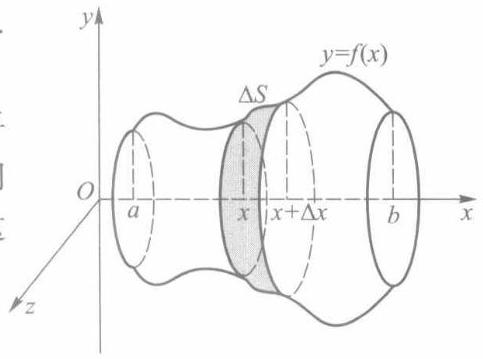
\includegraphics[width=.3\textwidth]{images/P085.jpg}
	\caption{图 $10-21$}
	\label{fig:P085}
\end{figure}

通过 \(x\) 轴上点 \(x\) 与 \(x + {\Delta x}\) 分别作垂直于 \(x\) 轴的平面, 它们在旋转曲面上截下一条夹在两个圆形截线间的狭带. 当 \({\Delta x}\) 很小时,此狭带的面积 \({\Delta S}\) 近似于由这两个圆所确定的圆台的侧面积 \({\Delta }^{\prime }S\) ,即
\[
{\Delta }^{\prime }S = \pi \left\lbrack  {f\left( x\right)  + f\left( {x + {\Delta x}}\right) }\right\rbrack  \sqrt{\Delta {x}^{2} + \Delta {y}^{2}}
\]
\[
= \pi \left\lbrack  {{2f}\left( x\right)  + {\Delta y}}\right\rbrack  \sqrt{1 + {\left( \frac{\Delta y}{\Delta x}\right) }^{2}}{\Delta x},
\]
其中 \({\Delta y} = f\left( {x + {\Delta x}}\right)  - f\left( x\right)\) . 由于
\[
\mathop{\lim }\limits_{{{\Delta x} \rightarrow  0}}{\Delta y} = 0,\mathop{\lim }\limits_{{{\Delta x} \rightarrow  0}}\sqrt{1 + {\left( \frac{\Delta y}{\Delta x}\right) }^{2}} = \sqrt{1 + {f}^{{\prime }^{2}}\left( x\right) },
\]


因此由 \({f}^{\prime }\left( x\right)\) 的连续性可以保证
\[
\pi \left\lbrack  {{2f}\left( x\right)  + {\Delta y}}\right\rbrack  \sqrt{1 + {\left( \frac{\Delta y}{\Delta x}\right) }^{2}}{\Delta x} - {2\pi f}\left( x\right) \sqrt{1 + {f}^{{\prime }^{2}}\left( x\right) }{\Delta x} = o\left( {\Delta x}\right) .
\]
所以得到
\[
{\Delta }^{\prime }S \approx  {2\pi f}\left( x\right) \sqrt{1 + {f}^{\prime 2}\left( x\right) }{\Delta x},
\]
\[
\mathrm{d}S = {2\pi f}\left( x\right) \sqrt{1 + {f}^{{\prime }^{2}}\left( x\right) }\mathrm{d}x,
\]
\[
S = {2\pi }{\int }_{a}^{b}f\left( x\right) \sqrt{1 + {f}^{{\prime }^{2}}\left( x\right) }\mathrm{d}x. \tag{3}
\]
如果光滑曲线 \(C\) 由参数方程
\[
x = x\left( t\right) ,y = y\left( t\right) ,t \in  \left\lbrack  {\alpha ,\beta }\right\rbrack
\]
给出,且 \(y\left( t\right)  \geq  0\) ,那么由弧微分知识推知曲线 \(C\) 绕 \(x\) 轴旋转所得旋转曲面的面积为
\[
S = {2\pi }{\int }_{\alpha }^{\beta }y\left( t\right) \sqrt{{x}^{\prime 2}\left( t\right)  + {y}^{\prime 2}\left( t\right) }\mathrm{d}t. \tag{4}
\]
%例 1
\begin{example}

\end{example}
计算圆 \({x}^{2} + {y}^{2} = {R}^{2}\) 在 \(\left\lbrack  {{x}_{1},{x}_{2}}\right\rbrack   \subset  \left\lbrack  {-R,R}\right\rbrack\) 上的弧段绕 \(x\) 轴旋转所得球带的面积.

%解
\begin{solution}

\end{solution}
对曲线 \(y = \sqrt{{R}^{2} - {x}^{2}}\) 在区间 \(\left\lbrack  {{x}_{1},{x}_{2}}\right\rbrack\) 上应用公式 (3),得到
\[
S = {2\pi }{\int }_{{x}_{1}}^{{x}_{2}}\sqrt{{R}^{2} - {x}^{2}}\sqrt{1 + \frac{{x}^{2}}{{R}^{2} - {x}^{2}}}\mathrm{\;d}x
\]
\[
= {2\pi R}{\int }_{{x}_{1}}^{{x}_{2}}\mathrm{\;d}x = {2\pi R}\left( {{x}_{2} - {x}_{1}}\right) .
\]
特别当 \({x}_{1} =  - R,{x}_{2} = R\) 时,得球的表面积 \({S}_{\text{ 球 }} = {4\pi }{R}^{2}\) .

%例 2
\begin{example}

\end{example}
计算由内摆线 \(x = a{\cos }^{3}t,y = a{\sin }^{3}t\) (见图 10-8) 绕 \(x\) 轴旋转所得旋转曲面的面积.

%解
\begin{solution}

\end{solution}
由曲线关于 \(y\) 轴的对称性及公式 (4),得
\[
S = {4\pi }{\int }_{0}^{\frac{\pi }{2}}{a{\sin }^{3}t\sqrt{{\left( {-{3a}{\cos }^{2}t\sin t}\right) }^{2} + {\left( {{3a}{\sin }^{2}t\cos t}\right) }^{2}}\mathrm{\;d}t}
\]
\[
= {12\pi }{a}^{2}{\int }_{0}^{\frac{\pi }{2}}{\sin }^{4}t\cos t\mathrm{\;d}t = \frac{12}{5}\pi {a}^{2}.
\]
\subsection{习题 10.4}

1. 求下列平面曲线绕指定轴旋转所得旋转曲面的面积:

(1) \(y = \sin x,0 \leq  x \leq  \pi\) ,绕 \(x\) 轴；

(2) \(x = a\left( {t - \sin t}\right) ,y = a\left( {1 - \cos t}\right) \left( {a > 0}\right) ,0 \leq  t \leq  {2\pi }\) ,绕 \(x\) 轴；

(3) \(\frac{{x}^{2}}{{a}^{2}} + \frac{{y}^{2}}{{b}^{2}} = 1\) ,绕 \(y\) 轴;

(4) \({x}^{2} + {\left( y - a\right) }^{2} = {r}^{2}\left( {r < a}\right)\) ,绕 \(x\) 轴.

2. 设平面光滑曲线由极坐标方程
\[
r = r\left( \theta \right) ,\alpha  \leq  \theta  \leq  \beta \left( {\left\lbrack  {\alpha ,\beta }\right\rbrack   \subset  \left\lbrack  {0,\pi }\right\rbrack  ,r\left( \theta \right)  \geq  0}\right)
\]
给出, 试求它绕极轴旋转所得旋转曲面的面积计算公式.

3. 试求下列极坐标曲线绕极轴旋转所得旋转曲面的面积:

(1)心形线 \(r = a\left( {1 + \cos \theta }\right) \left( {a > 0}\right)\) ；

(2)双纽线 \({r}^{2} = 2{a}^{2}\cos {2\theta }\left( {a > 0}\right)\) .

4. 证明: 如果在旋转曲面的面积公式 (3) 的推导过程中,过点 \(\left( {x,f\left( x\right) }\right)\) 作曲线 \(C\) 的切线,选取该切线在 \(\left\lbrack  {x,x + {\Delta x}}\right\rbrack\) 的一段绕 \(x\) 轴旋转一周生成圆台的侧面面积作为 \({\Delta S}\) 的近似可求量 \({\Delta }^{\prime }S\) ,则也可以得到公式 (3).

\section{定积分在物理中的某些应用}

定积分在物理中有着广泛的应用, 这里介绍几个较有代表性的例子.

\subsection{液体静压力}

%例 1
\begin{example}

\end{example}
如图10-22所示为一管道的圆形闸门 (半径为 \(3\mathrm{\;m}\) ). 问水平面齐及直径时, 闸门所受到的水的静压力为多大?

%解
\begin{solution}

\end{solution}
为方便起见,取 \(x\) 轴和 \(y\) 轴如图,此时圆的方程为
\[
{x}^{2} + {y}^{2} = 9\text{ . }
\]
由于在相同深度处水的静压强相同,其值等于 \({\rho gx}\) ,其中 \(\rho\) 为水的密度, \(g\) 为重力加速度, \(x\) 为深度,故当 \({\Delta x}\) 很小时,闸门上从深度 \(x\) 到 \(x + {\Delta x}\) 这一狭条 \({\Delta A}\) 上所受的静压力为
\[
{\Delta P} \approx  \mathrm{d}P = {2\rho gx}\sqrt{9 - {x}^{2}}\mathrm{\;d}x.
\]
从而闸门上所受的总压力为
\[
P = {\int }_{0}^{3}{2\rho gx}\sqrt{9 - {x}^{2}}\mathrm{\;d}x = {18\rho g}.
\]
\begin{figure}
	\centering
	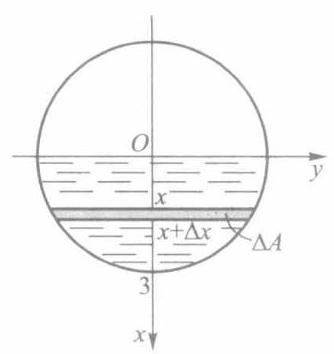
\includegraphics[width=.3\textwidth]{images/P086.jpg}
	\caption{图 $10-22$}
	\label{fig:P086}
\end{figure}

\begin{figure}
	\centering
	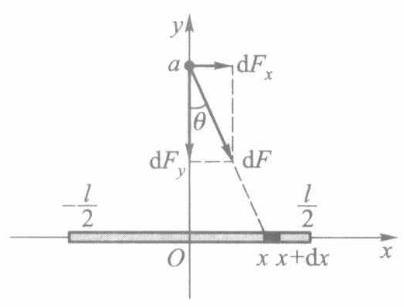
\includegraphics[width=.3\textwidth]{images/P087.jpg}
	\caption{图 $10-23$}
	\label{fig:P087}
\end{figure}

\subsection{引力}

%例 2
\begin{example}

\end{example}
一根长为 \(l\) 的均匀细杆,质量为 \(M\) ,在其中垂线上相距细杆为 \(a\) 处有一质量为 \(m\) 的质点. 试求细杆对质点的万有引力.

%解
\begin{solution}

\end{solution}
如图 10-23 所示,细杆位于 \(x\) 轴上的 \(\left\lbrack  {-\frac{l}{2},\frac{l}{2}}\right\rbrack\) ,质点位于 \(y\) 轴上的点 \(a\) . 任取 \(\left\lbrack  {x,x + {\Delta x}}\right\rbrack   \subset  \left\lbrack  {-\frac{l}{2},\frac{l}{2}}\right\rbrack\) ,当 \({\Delta x}\) 很小时可把这一小段细杆看作一质点,其质量为 \(\mathrm{d}M =\)  \(\frac{M}{l}\mathrm{\;d}x\) . 于是它对质点 \(m\) 的引力为
\[
\mathrm{d}F = \frac{{Gm}\mathrm{\;d}M}{{r}^{2}} = \frac{Gm}{{a}^{2} + {x}^{2}} \cdot  \frac{M}{l}\mathrm{\;d}x,
\]
其中 \(G\) 为万有引力常量. 由于细杆上各点对质点 \(m\) 的引力方向各不相同,因此不能直接对 \(\mathrm{d}F\) 进行积分 (不符合代数可加的条件). 为此,将 \(\mathrm{d}F\) 分解到 \(x\) 轴和 \(y\) 轴两个方向上,得
\[
\mathrm{d}{F}_{x} = \mathrm{d}F \cdot  \sin \theta ,\mathrm{d}{F}_{y} =  - \mathrm{d}F \cdot  \cos \theta .
\]
由于质点 \(m\) 位于细杆的中垂线上,必使水平合力为零,即
\[
{F}_{x} = {\int }_{-l/2}^{l/2}\mathrm{\;d}{F}_{x} = 0.
\]
又由 \(\cos \theta  = \frac{a}{\sqrt{{a}^{2} + {x}^{2}}}\) ,得垂直方向合力为
\[
{F}_{y} = {\int }_{-l/2}^{l/2}\mathrm{\;d}{F}_{y} =  - 2{\int }_{0}^{\frac{l}{2}}\frac{GmMa}{l}{\left( {a}^{2} + {x}^{2}\right) }^{-3/2}\mathrm{\;d}x
\]
\[
=  - {\left. \frac{2GmMa}{l} \cdot  \frac{1}{{a}^{2}} \cdot  \frac{x}{\sqrt{{a}^{2} + {x}^{2}}}\right| }_{0}^{l/2}
\]
\[
=  - \frac{2GmM}{a\sqrt{4{a}^{2} + {l}^{2}}},
\]
负号表示合力方向与 \(y\) 轴方向相反.

%例 3
\begin{example}

\end{example}
设有一半径为 \(r\) 的圆弧形导线,均匀带电,电荷密度为 \(\delta\) ,在圆心正上方距圆弧所在平面为 \(a\) 的地方有一电量为 \(q\) 的点电荷. 试求圆弧形导线与点电荷之间作用力 (引力或斥力)的大小.

%解
\begin{solution}

\end{solution}
如图 10-24 所示,把点电荷置于原点, \(z\) 轴垂直向下,圆弧形导线置于水平平面 \(z = a\) 上.

\begin{figure}
	\centering
	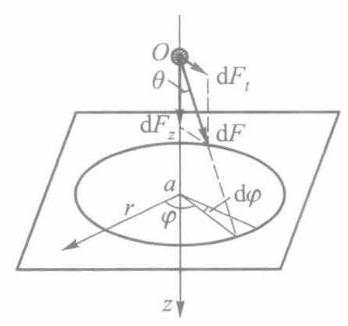
\includegraphics[width=.3\textwidth]{images/P088.jpg}
	\caption{图 $10-24$}
	\label{fig:P088}
\end{figure}

根据库仑定律,电量为 \({q}_{1},{q}_{2}\) 的两个点电荷之间的作用力 (引力或斥力) 的大小为
\[
F = \frac{k{q}_{1}{q}_{2}}{{\rho }^{2}},
\]
其中 \(\rho\) 是两点电荷之间的距离, \(k\) 是库仑常数.

把中心角为 \(\mathrm{d}\varphi\) 的一小段导线圆弧看作一点电荷,其电量为
\[
\mathrm{d}Q = \delta \mathrm{d}s = {\delta r}\mathrm{\;d}\varphi .
\]
它对点电荷 \(q\) 的作用力为
\[
\mathrm{d}F = k \cdot  \frac{q\mathrm{\;d}Q}{{\rho }^{2}} = \frac{k\delta rq}{{a}^{2} + {r}^{2}}\mathrm{\;d}\varphi .
\]
把 \(\mathrm{d}F\) 分解为 \(z\) 轴方向的垂直分力 \(\mathrm{d}{F}_{z}\) 和水平方向的分力 \(\mathrm{d}{F}_{t}\) . 由于点电荷位于圆弧导线的对称轴 \({Oz}\) 上,且导线上的电荷密度恒为常数,因此水平分力 \(\mathrm{d}{F}_{t}\) 各向抵消. 而
\[
\mathrm{d}{F}_{z} = \mathrm{d}F \cdot  \cos \theta  = \mathrm{d}F \cdot  \frac{a}{\sqrt{{a}^{2} + {r}^{2}}} = {k\delta raq}{\left( {a}^{2} + {r}^{2}\right) }^{-3/2}\mathrm{\;d}\varphi ,
\]
于是垂直方向的合力为
\[
{F}_{z} = {\int }_{0}^{2\pi }\mathrm{d}{F}_{z} = \frac{2\pi k\delta raq}{{\left( {a}^{2} + {r}^{2}\right) }^{3/2}}.
\]
这就是圆弧形导线与点电荷之间作用力的大小.

\subsection{功与平均功率}

%例 4
\begin{example}

\end{example}
一圆锥形水池,池口直径 \({30}\mathrm{\;m}\) ,深 \({20}\mathrm{\;m}\) ,池中盛满了水. 试求将全部池水抽出池外需做的功.

%解
\begin{solution}

\end{solution}
为方便起见, 取坐标轴如图 10-25 所示. 由于抽出相同深度处单位体积的水需做相同的功,因此首先考虑将池中深度为 \(x\) 到 \(x + {\Delta x}\) 的一薄层水 \({\Delta \Omega }\) 抽至池口需做的功 \({\Delta W}\) . 当 \({\Delta x}\) 很小时,把这一薄层水的深度都看作 \(x\) ,并取 \({\Delta \Omega }\) 的体积
\[
{\Delta V} \approx  \pi {\left\lbrack  {15}\left( 1 - \frac{x}{20}\right) \right\rbrack  }^{2}{\Delta x},
\]
这时有
\[
{\Delta W} \approx  \mathrm{d}W = {\pi \rho gx}{\left\lbrack  {15}\left( 1 - \frac{x}{20}\right) \right\rbrack  }^{2}\mathrm{\;d}x.
\]
从而将全部池水抽出池外需做的功为
\[
W = {225\pi \rho g}{\int }_{0}^{20}x{\left( 1 - \frac{x}{20}\right) }^{2}\mathrm{\;d}x = {7500\pi \rho g}.
\]
\begin{figure}
	\centering
	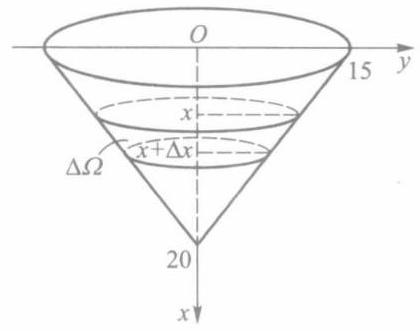
\includegraphics[width=.3\textwidth]{images/P089.jpg}
	\caption{图 $10-25$}
	\label{fig:P089}
\end{figure}

\begin{figure}
	\centering
	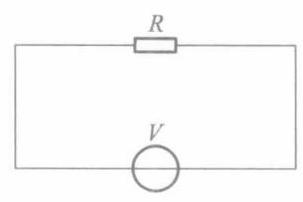
\includegraphics[width=.3\textwidth]{images/P090.jpg}
	\caption{图 $10-26$}
	\label{fig:P090}
\end{figure}

%例 5
\begin{example}

\end{example}
在纯电阻电路 (图 10-26) 中, 已知交流电压为
\[
V = {V}_{\mathrm{m}}\sin {\omega t}.
\]
求在一个周期 \(\left\lbrack  {0,T}\right\rbrack  \left( {T = \frac{2\pi }{\omega }}\right)\) 上消耗在电阻 \(R\) 上的能量 \(W\) ,并求与之相当的直流电压.

%解
\begin{solution}

\end{solution}
在直流电压 \(\left( {V = {V}_{0}}\right)\) 下,功率 \(P = \frac{{V}_{0}^{2}}{R}\) ,那么在时间 \(T\) 内所做的功为 \(W = {PT} = \frac{{V}_{0}^{2}T}{R}\) . 现在 \(V\) 为交流电压,瞬时功率为
\[
P\left( t\right)  = \frac{{V}_{\mathrm{m}}^{2}}{R}{\sin }^{2}{\omega t}.
\]
这相当于: 在任意一小段时间区间 \(\left\lbrack  {t,t + {\Delta t}}\right\rbrack   \subset  \left\lbrack  {0,T}\right\rbrack\) 上,当 \({\Delta t}\) 很小时,可把 \(V\) 近似看作恒为 \({V}_{\mathrm{m}}\sin {\omega t}\) 的情形. 于是取功的微元为
\[
\mathrm{d}W = P\left( t\right) \mathrm{d}t.
\]
并由此求得
\[
W = {\int }_{0}^{T}P\left( t\right) \mathrm{d}t = {\int }_{0}^{\frac{2\pi }{\omega }}\frac{{V}_{\mathrm{m}}^{2}}{R}{\sin }^{2}{\omega t}\mathrm{\;d}t = \frac{\pi {V}_{\mathrm{m}}^{2}}{R\omega }.
\]
而平均功率则为
\[
\bar{P} = \frac{1}{T}{\int }_{0}^{T}P\left( t\right) \mathrm{d}t = \frac{\omega }{2\pi } \cdot  \frac{\pi {V}_{\mathrm{m}}^{2}}{R\omega } = \frac{{V}_{\mathrm{m}}^{2}}{2R} = \frac{{\left( {V}_{\mathrm{m}}/\sqrt{2}\right) }^{2}}{R}.
\]
上述结果的最末形式,表示交流电压 \(V = {V}_{\mathrm{m}}\sin {\omega t}\) 在一个周期上的平均功率与直流电压 \(\bar{V} = \frac{{V}_{m}}{\sqrt{2}}\) 的功率是相等的. 故称 \(\bar{V}\) 为该交流电压的有效值. 通常所说的 \({220}\mathrm{\;V}\) 交流电,其实是 \(V = {220}\sqrt{2}\sin {\omega t}\) 的有效值.

\subsection{习题 10.5}

1. 有一等腰梯形闸门,它的上、下两条底边各长为 \({10}\mathrm{\;m}\) 和 \(6\mathrm{\;m}\) ,高为 \({20}\mathrm{\;m}\) . 计算当水面与上底边相齐时闸门一侧所受的静压力.

2. 边长为 \(a\) 和 \(b\) 的矩形薄板,与液面成 \(\alpha \left( {0 < \alpha  < {90}^{ \circ  }}\right)\) 角斜沉于液体中. 设 \(a > b\) ,长边平行于液面, 上沿位于深 \(h\) 处,液体的比重为 \(\nu\) . 试求薄板每侧所受的静压力.

3. 直径为 \(6\mathrm{\;m}\) 的一球浸入水中,其球心在水平面下 \({10}\mathrm{\;m}\) 处,求球面上所受浮力.

4. 设在坐标轴的原点有一质量为 \(m\) 的质点,在区间 \(\left\lbrack  {a,a + l}\right\rbrack  \left( {a > 0}\right)\) 上有一质量为 \(M\) 的均匀细杆. 试求质点与细杆之间的万有引力.

5. 设有两条各长为 \(l\) 的均匀细杆在同一直线上,中间离开距离 \(c\) ,每根细杆的质量为 \(M\) . 试求它们之间的万有引力. (提示: 在第 4 题的基础上再作一次积分. )

6. 设有半径为 \(r\) 的半圆形导线,均匀带电,电荷密度为 \(\delta\) ,在圆心处有一单位正电荷. 试求它们之间作用力的大小.

7. 一个半球形 (直径为 \({20}\mathrm{\;m}\) ) 的容器内盛满了水. 试问把水抽尽需做多少功?

8. 长 \({10}\mathrm{\;m}\) 的铁索下垂于矿井中,已知铁索每米的质量为 \(8\mathrm{\;{kg}}\) ,问将此铁索提出地面需做多少功?

9. 一物体在某介质中按 \(x = c{t}^{3}\) 作直线运动,介质的阻力与速度 \(\frac{\mathrm{d}x}{\mathrm{\;d}t}\) 的平方成正比. 计算物体由 \(x =\) 0 移至 \(x = a\) 时克服介质阻力所做的功.

10. 半径为 \(r\) 的球体沉入水中,其比重与水相同. 试问将球体从水中捞出需做多少功?

\section{* §6 定积分的近似计算}

利用牛顿一莱布尼茨公式虽然可以精确地计算定积分的值, 但它仅适用于被积函数的原函数能够求得的情形. 如果这点办不到或者不容易办到, 这就要考虑近似计算的方法. 在定积分的很多应用问题中, 被积函数甚至没有解析表达式 (只是一条实验记录曲线,或者是一组离散的采样值),这时只能采用近似方法去计算相应的定积分。

其实, 根据定积分的定义, 每一个积分和都可看做是定积分的一个近似值, 例如
\[
{\int }_{a}^{b}f\left( x\right) \mathrm{d}x \approx  \mathop{\sum }\limits_{{i = 1}}^{n}f\left( {x}_{i}\right) \Delta {x}_{i}\left( \right. \text{ 或 }\left. {\mathop{\sum }\limits_{{i = 1}}^{n}f\left( {x}_{i - 1}\right) \Delta {x}_{i}}\right) \text{ . } \tag{1}
\]
在几何意义上, 这是用一系列小矩形面积来近似小曲边梯形面积的结果. 所以把这个近似算法称为矩形法. 不过, 只有当积分区间被分割得很细很细时, 矩形法才有一定的精确度.

如果在分割的每个小区间上采用一次或二次多项式来近似替代被积函数, 那么可以期望获得比矩形法效果好得多的近似计算公式. 下面的梯形法和抛物线法就是这一想法的产物.

\subsection{梯形法}

将积分区间 \(\left\lbrack  {a,b}\right\rbrack\) 作 \(n\) 等分,分点依次为
\[
a = {x}_{0} < {x}_{1} < {x}_{2} < \cdots  < {x}_{n} = b,\Delta {x}_{i} = \frac{b - a}{n}.
\]
相应的被积函数值记为
\[
{y}_{0},{y}_{1},{y}_{2},\cdots ,{y}_{n}\left( {{y}_{i} = f\left( {x}_{i}\right) ,i = 0,1,2,\cdots ,n}\right) .
\]
并记曲线 \(y = f\left( x\right)\) 上相应的点为
\[
{P}_{0},{P}_{1},{P}_{2},\cdots ,{P}_{n}\left( {{P}_{i}\left( {{x}_{i},{y}_{i}}\right) ,i = 0,1,2,\cdots ,n}\right) .
\]
将曲线上每一段弧 \(\overset{⏜}{{P}_{i - 1}{P}_{i}}\) 用弦 \(\overline{{P}_{i - 1}{P}_{i}}\) 来替代,这使得每个小区间 \(\left\lbrack  {{x}_{i - 1},{x}_{i}}\right\rbrack\) 上的曲边梯形换成了真正的梯形 (图 10-27), 其面积为
\[
\frac{{y}_{i - 1} + {y}_{i}}{2}\Delta {x}_{i},i = 1,2,\cdots ,n.
\]
于是,各个小梯形面积之和就是曲边梯形面积的近似值,即
\[
{\int }_{a}^{b}f\left( x\right) \mathrm{d}x \approx  \mathop{\sum }\limits_{{i = 1}}^{n}\frac{{y}_{i - 1} + {y}_{i}}{2}\Delta {x}_{i},
\]
亦即
\[
{\int }_{a}^{b}f\left( x\right) \mathrm{d}x \approx  \frac{b - a}{n}\left( {\frac{{y}_{0}}{2} + {y}_{1} + {y}_{2} + \cdots  + {y}_{n - 1} + \frac{{y}_{n}}{2}}\right) . \tag{2}
\]
称此近似式为定积分的梯形法公式.

\begin{figure}
	\centering
	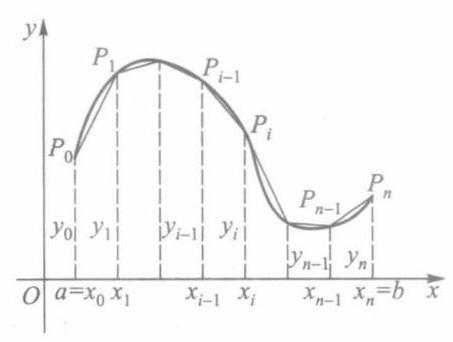
\includegraphics[width=.3\textwidth]{images/P091.jpg}
	\caption{图 $10-27$}
	\label{fig:P091}
\end{figure}

\begin{figure}
	\centering
	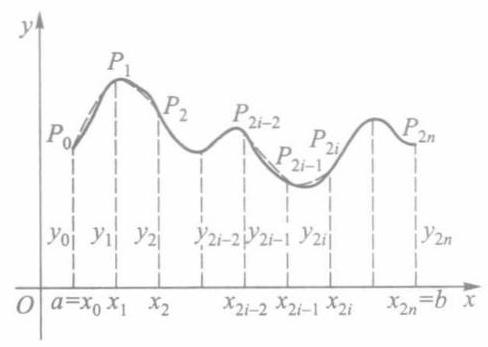
\includegraphics[width=.3\textwidth]{images/P092.jpg}
	\caption{图 $10-28$}
	\label{fig:P092}
\end{figure}

\subsection{抛物线法}

由梯形法求定积分的近似值,当 \(y = f\left( x\right)\) 为凸曲线时偏大,为凹曲线时偏小. 如果每段曲线改用与它的凸性相接近的抛物线来近似, 就可减少上述缺点. 下面介绍抛物线法.

将积分区间 \(\left\lbrack  {a,b}\right\rbrack\) 作 \({2n}\) 等分 (图 10-28),分点依次为
\[
a = {x}_{0} < {x}_{1} < {x}_{2} < \cdots  < {x}_{2n} = b,\Delta {x}_{i} = \frac{b - a}{2n}.
\]
对应的被积函数值为
\[
{y}_{0},{y}_{1},{y}_{2},\cdots ,{y}_{2n}\left( {{y}_{i} = f\left( {x}_{i}\right) ,i = 0,1,2,\cdots ,{2n}}\right) .
\]
曲线 \(y = f\left( x\right)\) 上的相应点为
\[
{P}_{0},{P}_{1},{P}_{2},\cdots ,{P}_{2n}\left( {{P}_{i}\left( {{x}_{i},{y}_{i}}\right) ,i = 0,1,2,\cdots ,{2n}}\right) .
\]
现把区间 \(\left\lbrack  {{x}_{0},{x}_{2}}\right\rbrack\) 上的曲线 \(y = f\left( x\right)\) 用通过三点
\[
{P}_{0}\left( {{x}_{0},{y}_{0}}\right) ,{P}_{1}\left( {{x}_{1},{y}_{1}}\right) ,{P}_{2}\left( {{x}_{2},{y}_{2}}\right)
\]
的抛物线 \({p}_{1}\left( x\right)  = {\alpha }_{1}{x}^{2} + {\beta }_{1}x + {\gamma }_{1}\) 来近似替代,便有
\[
{\int }_{{x}_{0}}^{{x}_{2}}f\left( x\right) \mathrm{d}x \approx  {\int }_{{x}_{0}}^{{x}_{2}}{p}_{1}\left( x\right) \mathrm{d}x = {\int }_{{x}_{0}}^{{x}_{2}}\left( {{\alpha }_{1}{x}^{2} + {\beta }_{1}x + {\gamma }_{1}}\right) \mathrm{d}x
\]
\[
= \frac{{\alpha }_{1}}{3}\left( {{x}_{2}^{3} - {x}_{0}^{3}}\right)  + \frac{{\beta }_{1}}{2}\left( {{x}_{2}^{2} - {x}_{0}^{2}}\right)  + {\gamma }_{1}\left( {{x}_{2} - {x}_{0}}\right)
\]
\[
= \frac{{x}_{2} - {x}_{0}}{6}\left\lbrack  {\left( {{\alpha }_{1}{x}_{0}^{2} + {\beta }_{1}{x}_{0} + {\gamma }_{1}}\right)  + \left( {{\alpha }_{1}{x}_{2}^{2} + {\beta }_{1}{x}_{2} + {\gamma }_{1}}\right)  + }\right.
\]
\[
\left. {{\alpha }_{1}{\left( {x}_{0} + {x}_{2}\right) }^{2} + 2{\beta }_{1}\left( {{x}_{0} + {x}_{2}}\right)  + 4{\gamma }_{1}}\right\rbrack
\]
\[
= \frac{{x}_{2} - {x}_{0}}{6}\left( {{y}_{0} + {y}_{2} + 4{y}_{1}}\right)  = \frac{b - a}{6n}\left( {{y}_{0} + 4{y}_{1} + {y}_{2}}\right) .
\]
倒数第二式的得来是利用了 \({x}_{0} + {x}_{2} = 2{x}_{1}\) .

同样地,在 \(\left\lbrack  {{x}_{{2i} - 2},{x}_{2i}}\right\rbrack\) 上用 \({p}_{i}\left( x\right)  = {\alpha }_{i}{x}^{2} + {\beta }_{i}x + {\gamma }_{i}\) 替代曲线 \(y = f\left( x\right)\) ,将得到
\[
{\int }_{{x}_{{2i} - 2}}^{{x}_{2i}}f\left( x\right) \mathrm{d}x \approx  {\int }_{{x}_{{2i} - 2}}^{{x}_{2i}}{p}_{i}\left( x\right) \mathrm{d}x = \frac{b - a}{6n}\left( {{y}_{{2i} - 2} + 4{y}_{{2i} - 1} + {y}_{2i}}\right) .
\]
最后,按 \(i = 1,2,\cdots ,n\) 把这些近似式相加,得到
\[
{\int }_{a}^{b}f\left( x\right) \mathrm{d}x = \mathop{\sum }\limits_{{i = 1}}^{n}{\int }_{{x}_{{2i} - 2}}^{{x}_{2i}}f\left( x\right) \mathrm{d}x \approx  \frac{b - a}{6n}\mathop{\sum }\limits_{{i = 1}}^{n}\left( {{y}_{{2i} - 2} + 4{y}_{{2i} - 1} + {y}_{2i}}\right) ,
\]
即
\[
{\int }_{a}^{b}f\left( x\right) \mathrm{d}x \approx  \frac{b - a}{6n}\left\lbrack  {{y}_{0} + {y}_{2n} + 4\left( {{y}_{1} + {y}_{3} + \cdots  + {y}_{{2n} - 1}}\right)  + }\right.
\]
\[
\left. {2\left( {{y}_{2} + {y}_{4} + \cdots  + {y}_{{2n} - 2}}\right) }\right\rbrack  \text{ . } \tag{3}
\]
这就是抛物线法公式, 也称为辛普森 (Simpson) 公式.

作为例子,我们计算定积分 \({\int }_{0}^{1}\frac{\mathrm{d}x}{1 + {x}^{2}}\) 的近似值.

将区间 \(\left\lbrack  {0,1}\right\rbrack\) 十等分,各分点上被积函数的值列表如下 (取七位小数):

\begin{center}
\adjustbox{max width=\textwidth}{
\begin{tabular}{|c|c|c|c|c|c|c|}
\hline
\({x}_{i}\) & 0 & 0.1 & 0.2 & 0.3 & 0.4 & 0.5 \\
\cline{1-7}
\({y}_{i}\) & 1 & 0.990 099 0 & 0.961 538 5 & 0.917 431 2 & 0.862 069 0 & 0.800 000 0 \\
\cline{1-7}
\({x}_{i}\) & 0.6 & 0.7 & 0.8 & 0.9 & 1 & \phantom{X} \\
\cline{1-7}
\({y}_{i}\) & 0.735 294 1 & 0.671 140 9 & 0.609 756 1 & 0.552 486 2 & 0.500 000 0 & \phantom{X} \\
\cline{1-7}
\hline
\end{tabular}
}
\end{center}

1) 用矩形法公式 (1) 去计算 (取四位小数):
\[
{\int }_{0}^{1}\frac{\mathrm{d}x}{1 + {x}^{2}} \approx  \frac{1}{10}\left( {{y}_{0} + {y}_{1} + \cdots  + {y}_{9}}\right)  \approx  {0.8100}
\]
\[
\text{ (或 }\frac{1}{10}\left( {{y}_{1} + {y}_{2} + \cdots  + {y}_{10}}\right)  \approx  {0.7600}\text{ ). }
\]
2)用梯形法公式(2)去计算(取四位小数):
\[
{\int }_{0}^{1}\frac{\mathrm{d}x}{1 + {x}^{2}} \approx  \frac{1}{10}\left( {\frac{{y}_{0}}{2} + {y}_{1} + {y}_{2} + \cdots  + {y}_{9} + \frac{{y}_{10}}{2}}\right)  \approx  {0.7850}.
\]
3)用抛物线法公式(3)去计算(取七位小数):
\[
{\int }_{0}^{1}\frac{\mathrm{d}x}{1 + {x}^{2}} \approx  \frac{1}{30}\left\lbrack  {{y}_{0} + {y}_{10} + 4\left( {{y}_{1} + {y}_{3} + \cdots  + {y}_{9}}\right)  + 2\left( {{y}_{2} + {y}_{4} + \cdots  + {y}_{8}}\right) }\right\rbrack
\]
\[
\approx  {0.7853982}\text{ . }
\]
用准确值\footnote{这里用一个很容易求得准确值的定积分作为近似计算的例子,主要的理由就是有准确值可以与近似值相比较. 实际使用中不会有这样的事.}
\[
{\int }_{0}^{1}\frac{\mathrm{d}x}{1 + {x}^{2}} = \arctan 1 = \frac{\pi }{4} = {0.78539816}\cdots
\]
与上述近似值相比较, 矩形法的结果只有一位有效数字是准确的, 梯形法的结果有三位有效数字是准确的, 抛物线法的结果则有六位有效数字是准确的. 可见公式 (3) 明显地优于公式 (2), 更优于公式 (1).

关于定积分近似计算的误差估计,在 “数值分析” 一类课程中必有详述,这里不再讨论.

\subsection{习题 10.6}

1. 分别用梯形法和抛物线法近似计算 \({\int }_{1}^{2}\frac{\mathrm{d}x}{x}\) (将积分区间十等分).



2. 用抛物线法近似计算 \({\int }_{0}^{\pi }\frac{\sin x}{x}\mathrm{\;d}x\) (分别将积分区间二等分、四等分、六等分).

3. 图 10-29 所示为河道某一截面图. 试由测得数据用抛物线法求截面面积.

\begin{figure}
	\centering
	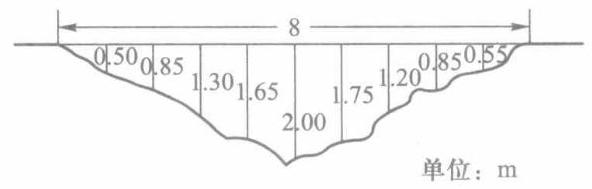
\includegraphics[width=.3\textwidth]{images/P093.jpg}
	\caption{图 $10-29$}
	\label{fig:P093}
\end{figure}

4. 下表所列为夏季某一天每隔两小时测得的气温:

\begin{center}
\adjustbox{max width=\textwidth}{
\begin{tabular}{|c|c|c|c|c|c|c|c|c|c|c|c|c|c|}
\hline
时间 \({t}_{i}\) & 0 & 2 & 4 & 6 & 8 & 10 & 12 & 14 & 16 & 18 & 20 & 22 & 24 \\
\cline{1-14}
温度 \({C}_{i}\) & 25.8 & 23.0 & 24.1 & 25.6 & 27.3 & 30.2 & 33.4 & 35.0 & 33.8 & 31.1 & 28.2 & 27.0 & 25.0 \\
\cline{1-14}
\hline
\end{tabular}
}
\end{center}

(1)按积分平均 \(\frac{1}{b - a}{\int }_{a}^{b}f\left( t\right) \mathrm{d}t\) 求这一天的平均气温,其中定积分值由三种近似法分别计算；

(2)若按算术平均 \(\frac{1}{12}\mathop{\sum }\limits_{{i = 1}}^{{12}}{C}_{i - 1}\) 或 \(\frac{1}{12}\mathop{\sum }\limits_{{i = 1}}^{{12}}{C}_{i}\) 求得平均气温,那么它们与矩形法积分平均和梯形法积分平均各有什么联系? 简述理由.

